\chapter{Моделирование}
\label{ch:chap3}


\section{Визуализация}

\begin{figure}[h]
\center{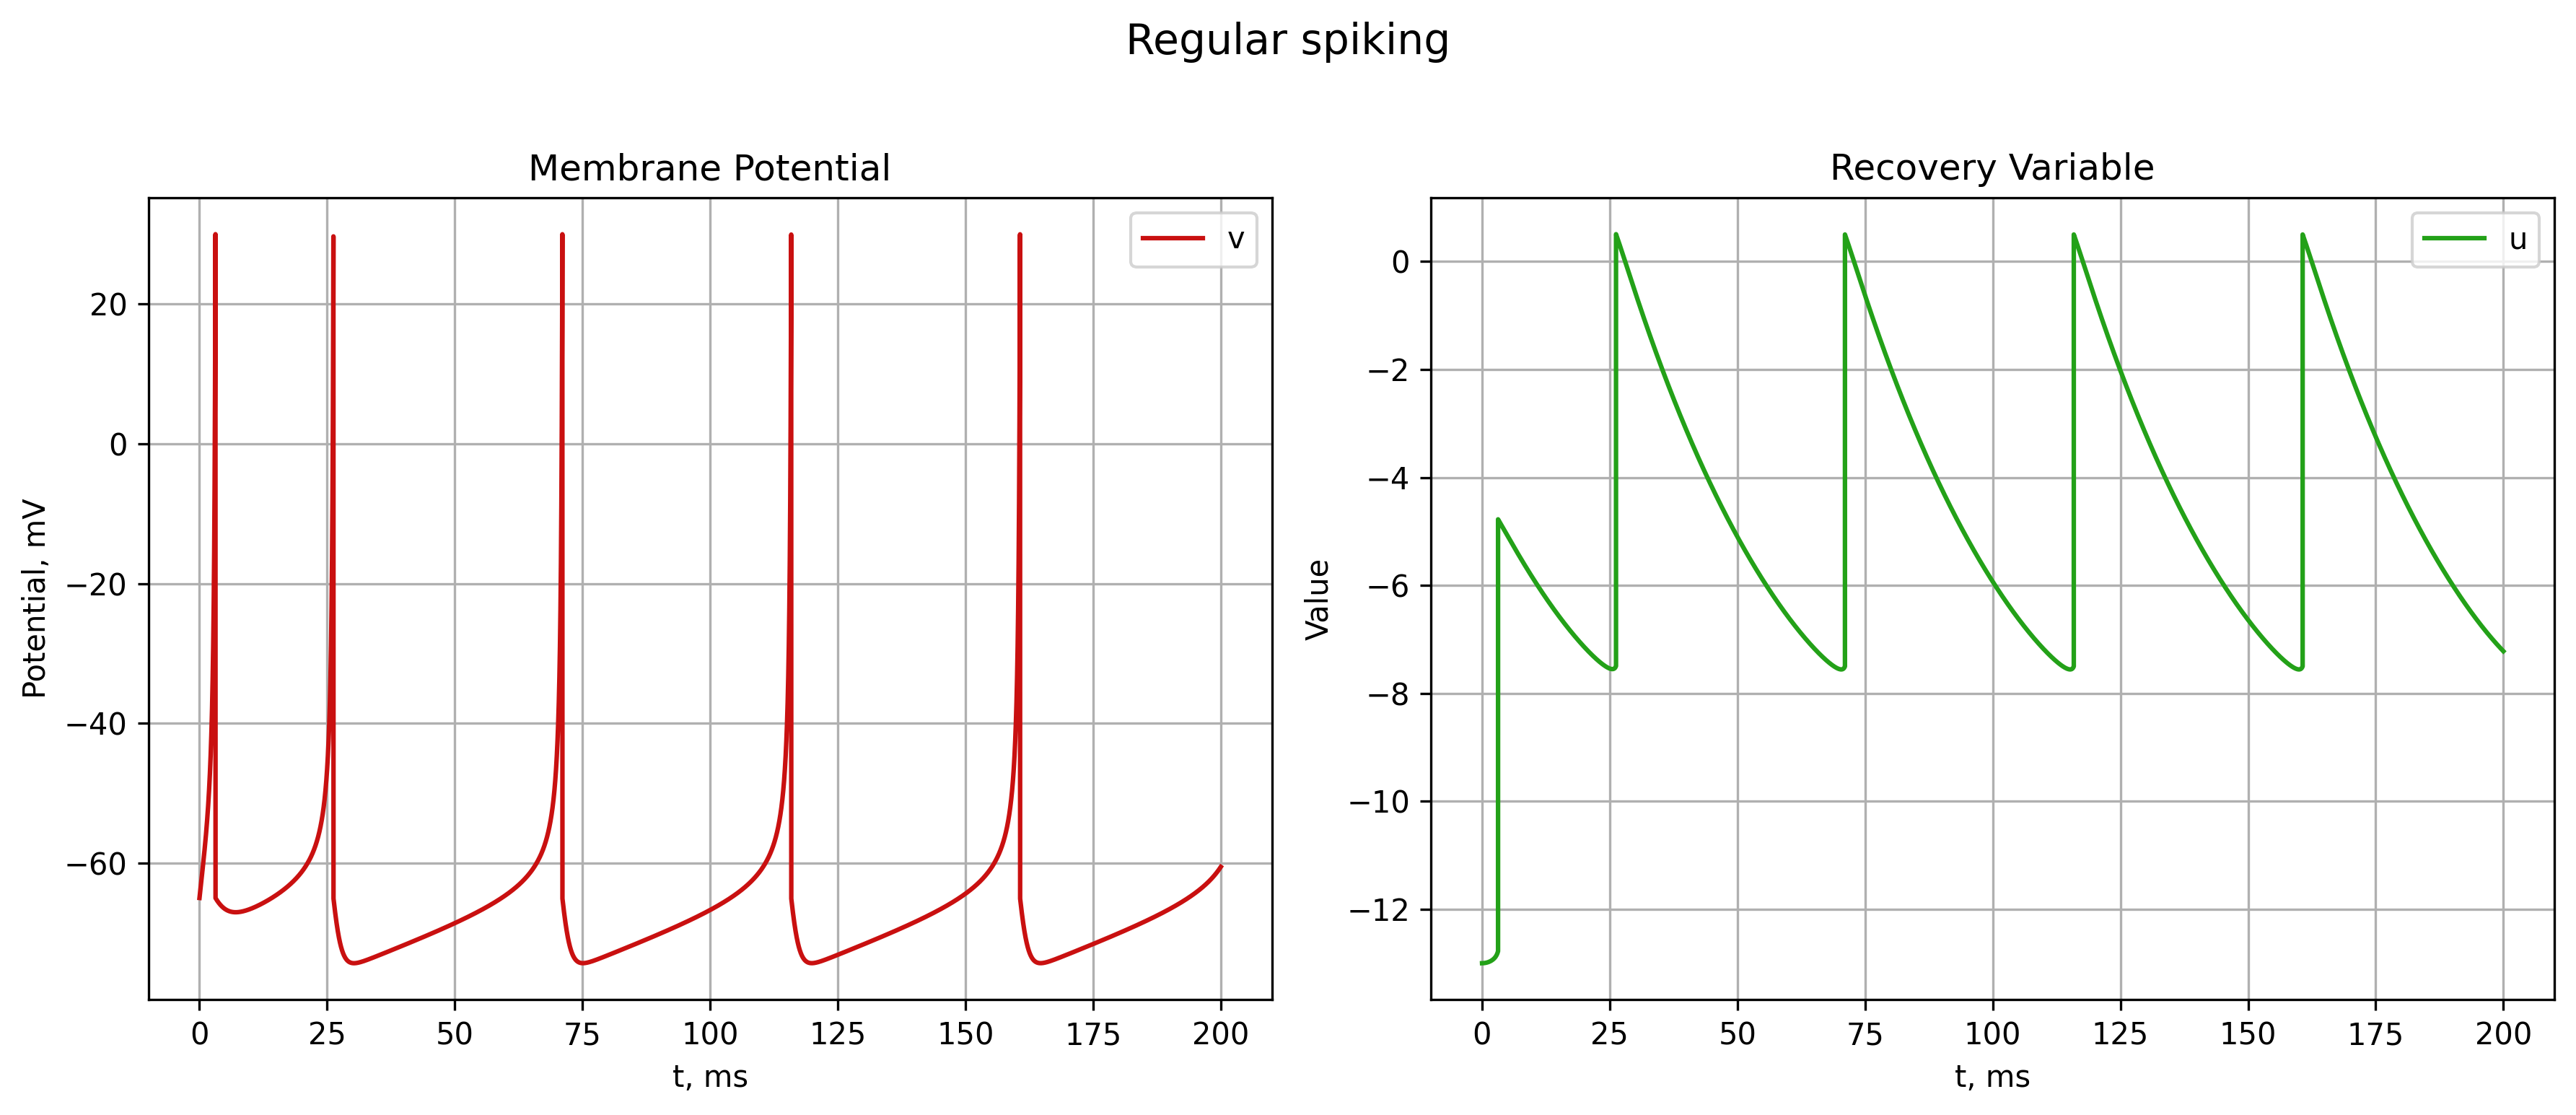
\includegraphics[width=1\linewidth]{pic/regular_spiking.png}}
\caption{Визуализация регулярно-спайкового нейрона при $I=10$ нА.}
\label{1_rs}
\end{figure}

\begin{figure}[h]
	\center{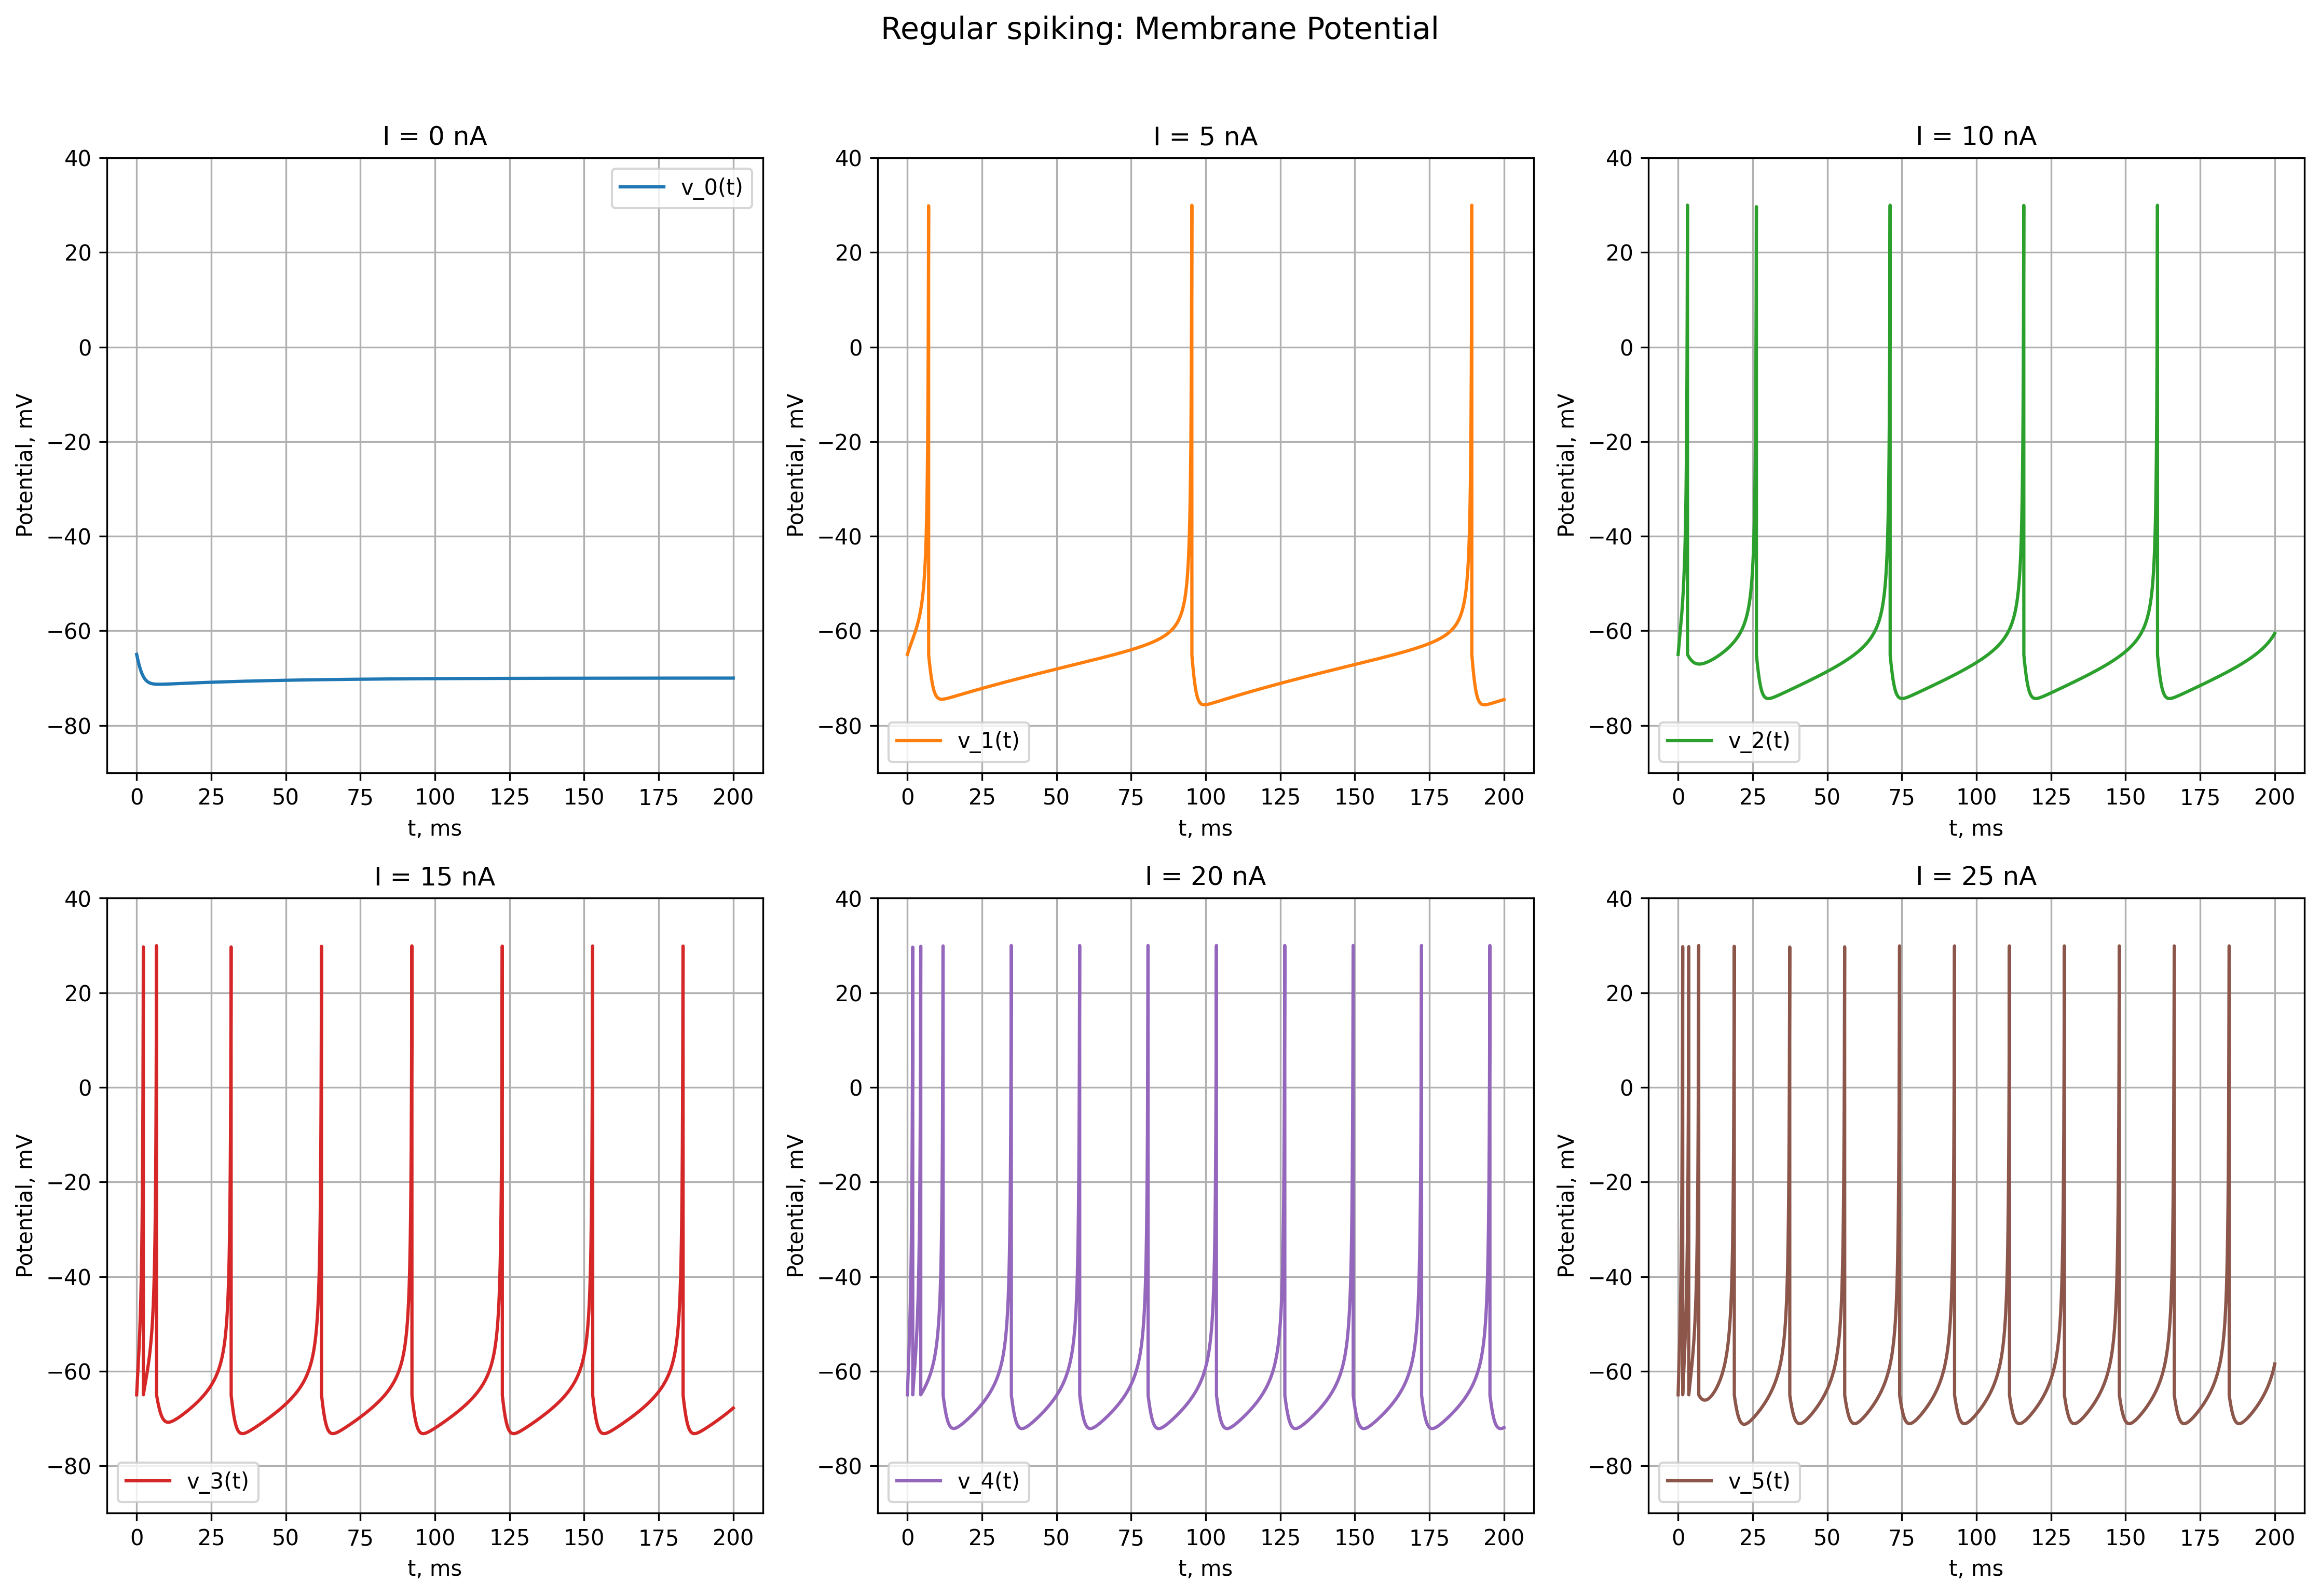
\includegraphics[width=1\linewidth]{pic/rs_different_I_potentials.png}}
	\caption{Визуализация $v(t)$ регулярно-спайкового нейрона для разных значений $I$.}
	\label{rs_different_I_potentials}
\end{figure}

\begin{figure}[h]
	\center{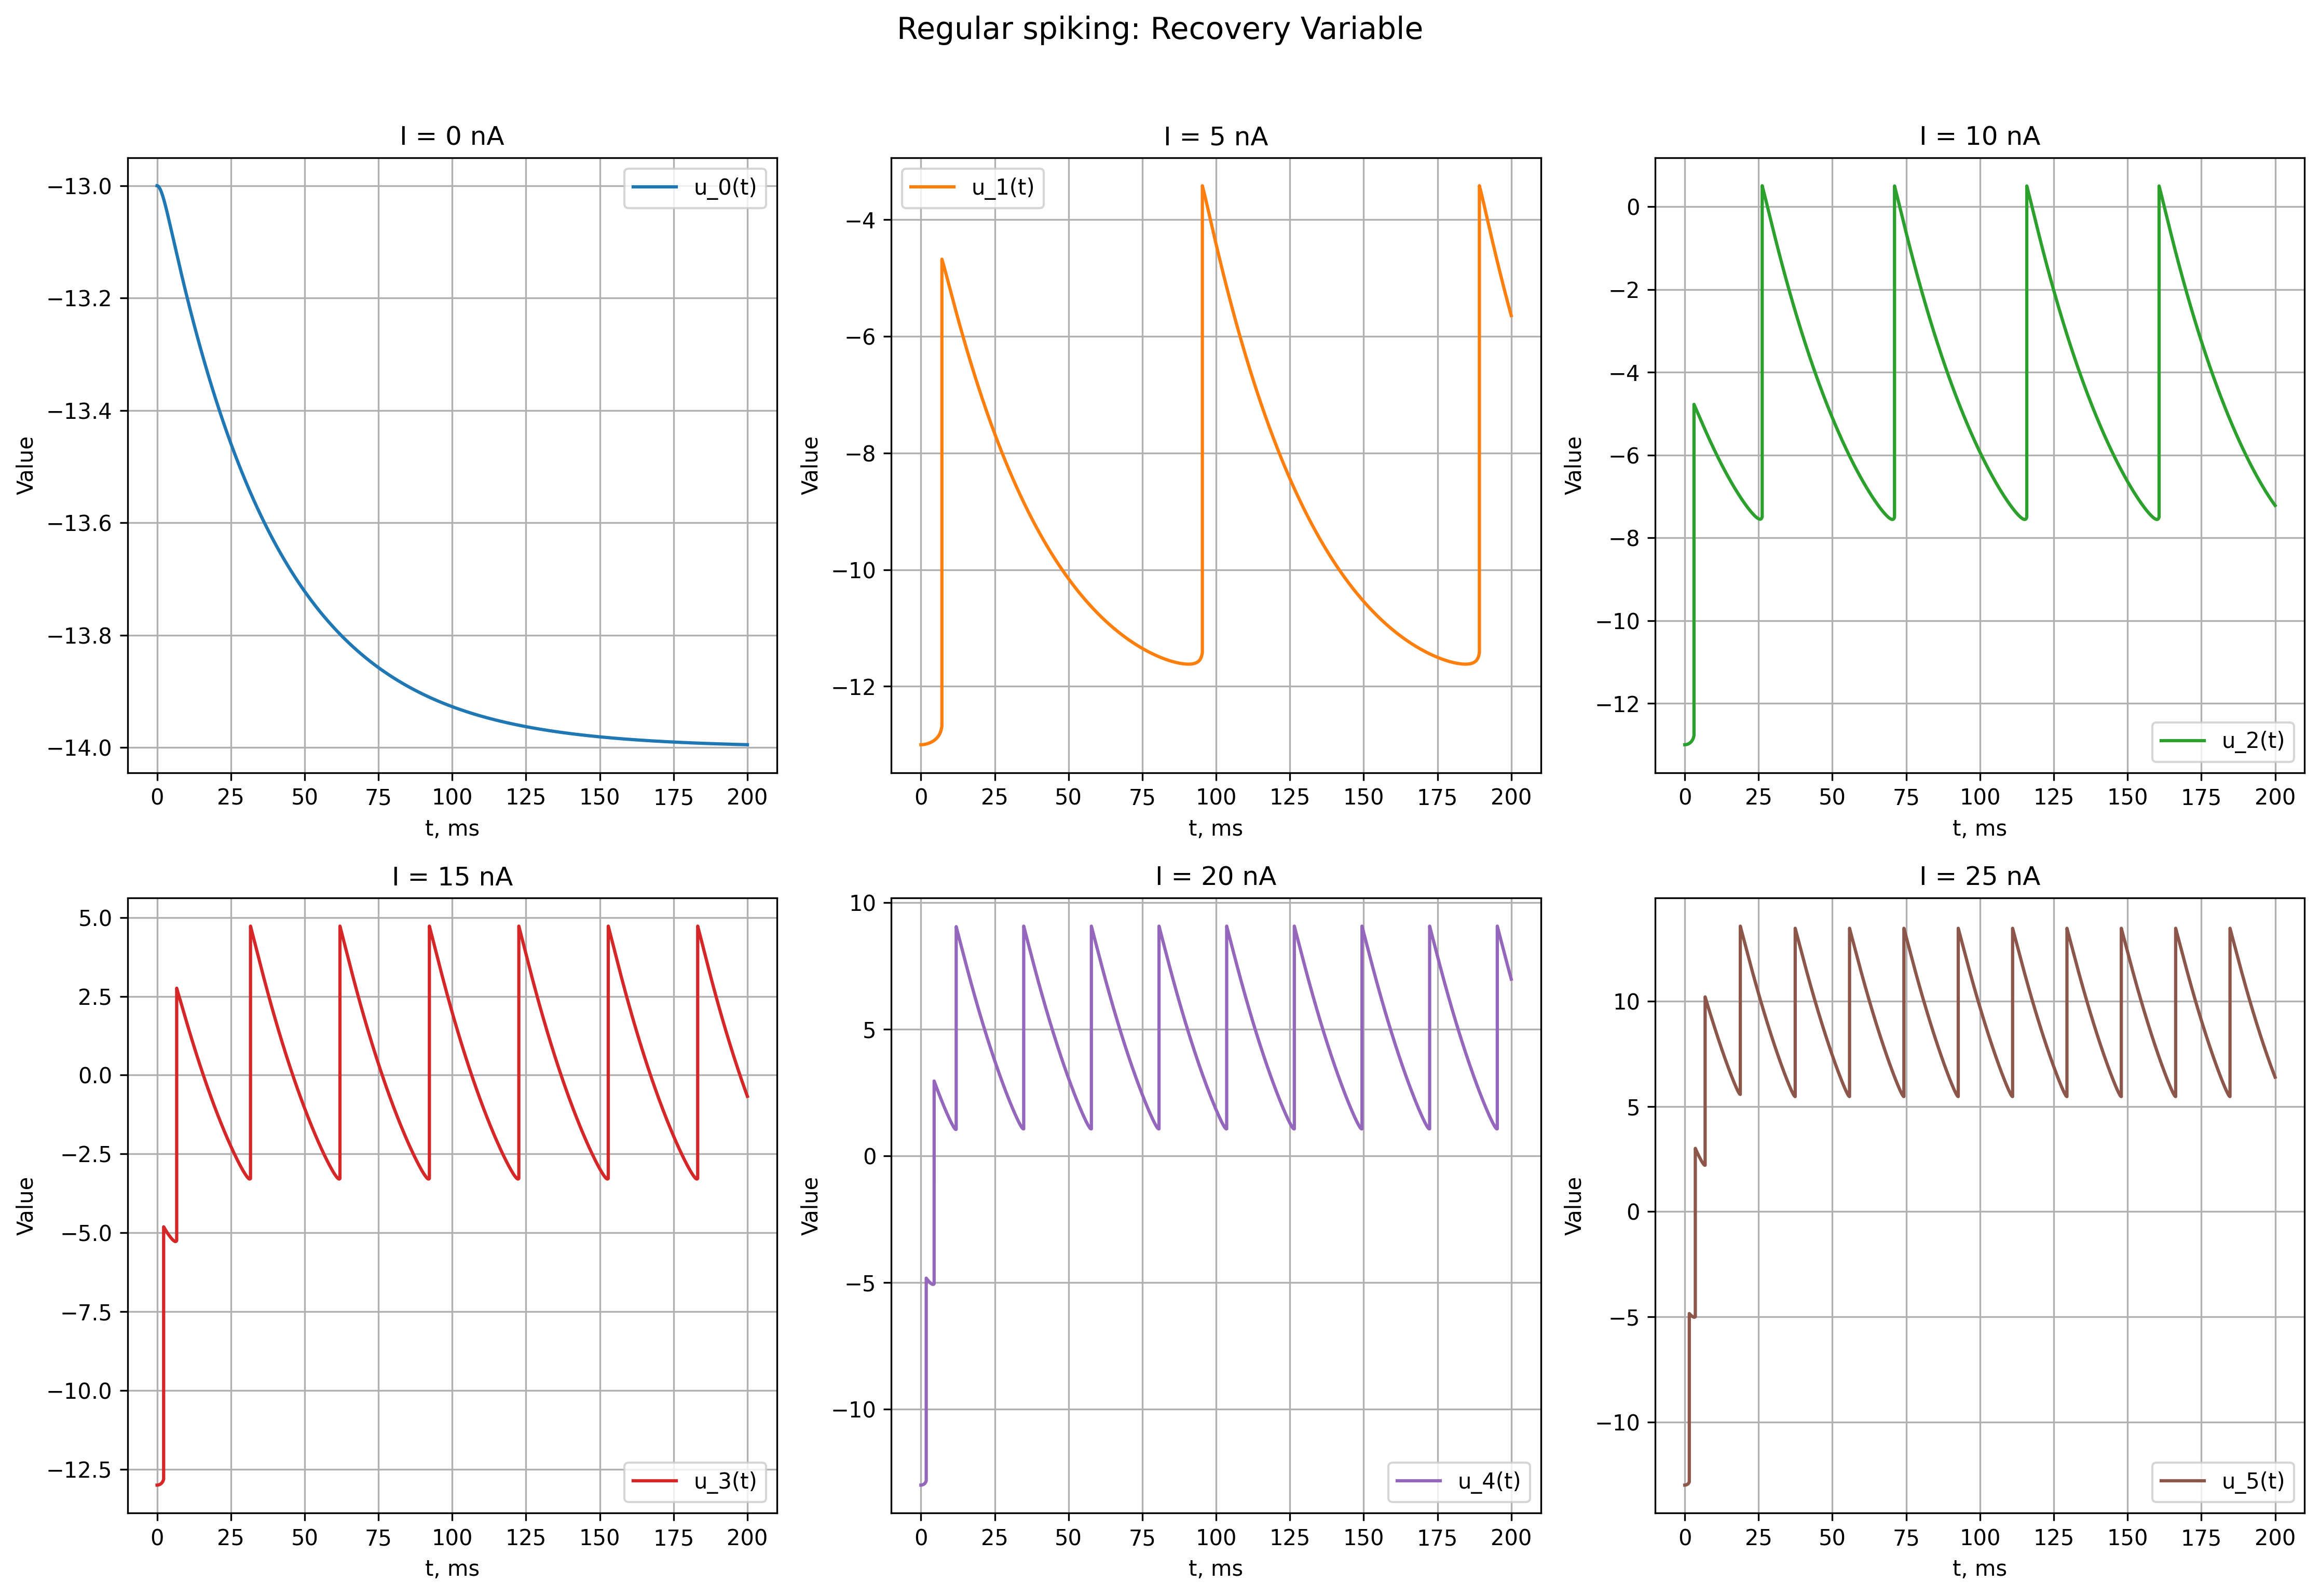
\includegraphics[width=1\linewidth]{pic/rs_different_I_recovery.png}}
	\caption{Визуализация $u(t)$ регулярно-спайкового нейрона для разных значений $I$.}
	\label{rs_different_I_recovery}
\end{figure}

\begin{figure}[h]
\center{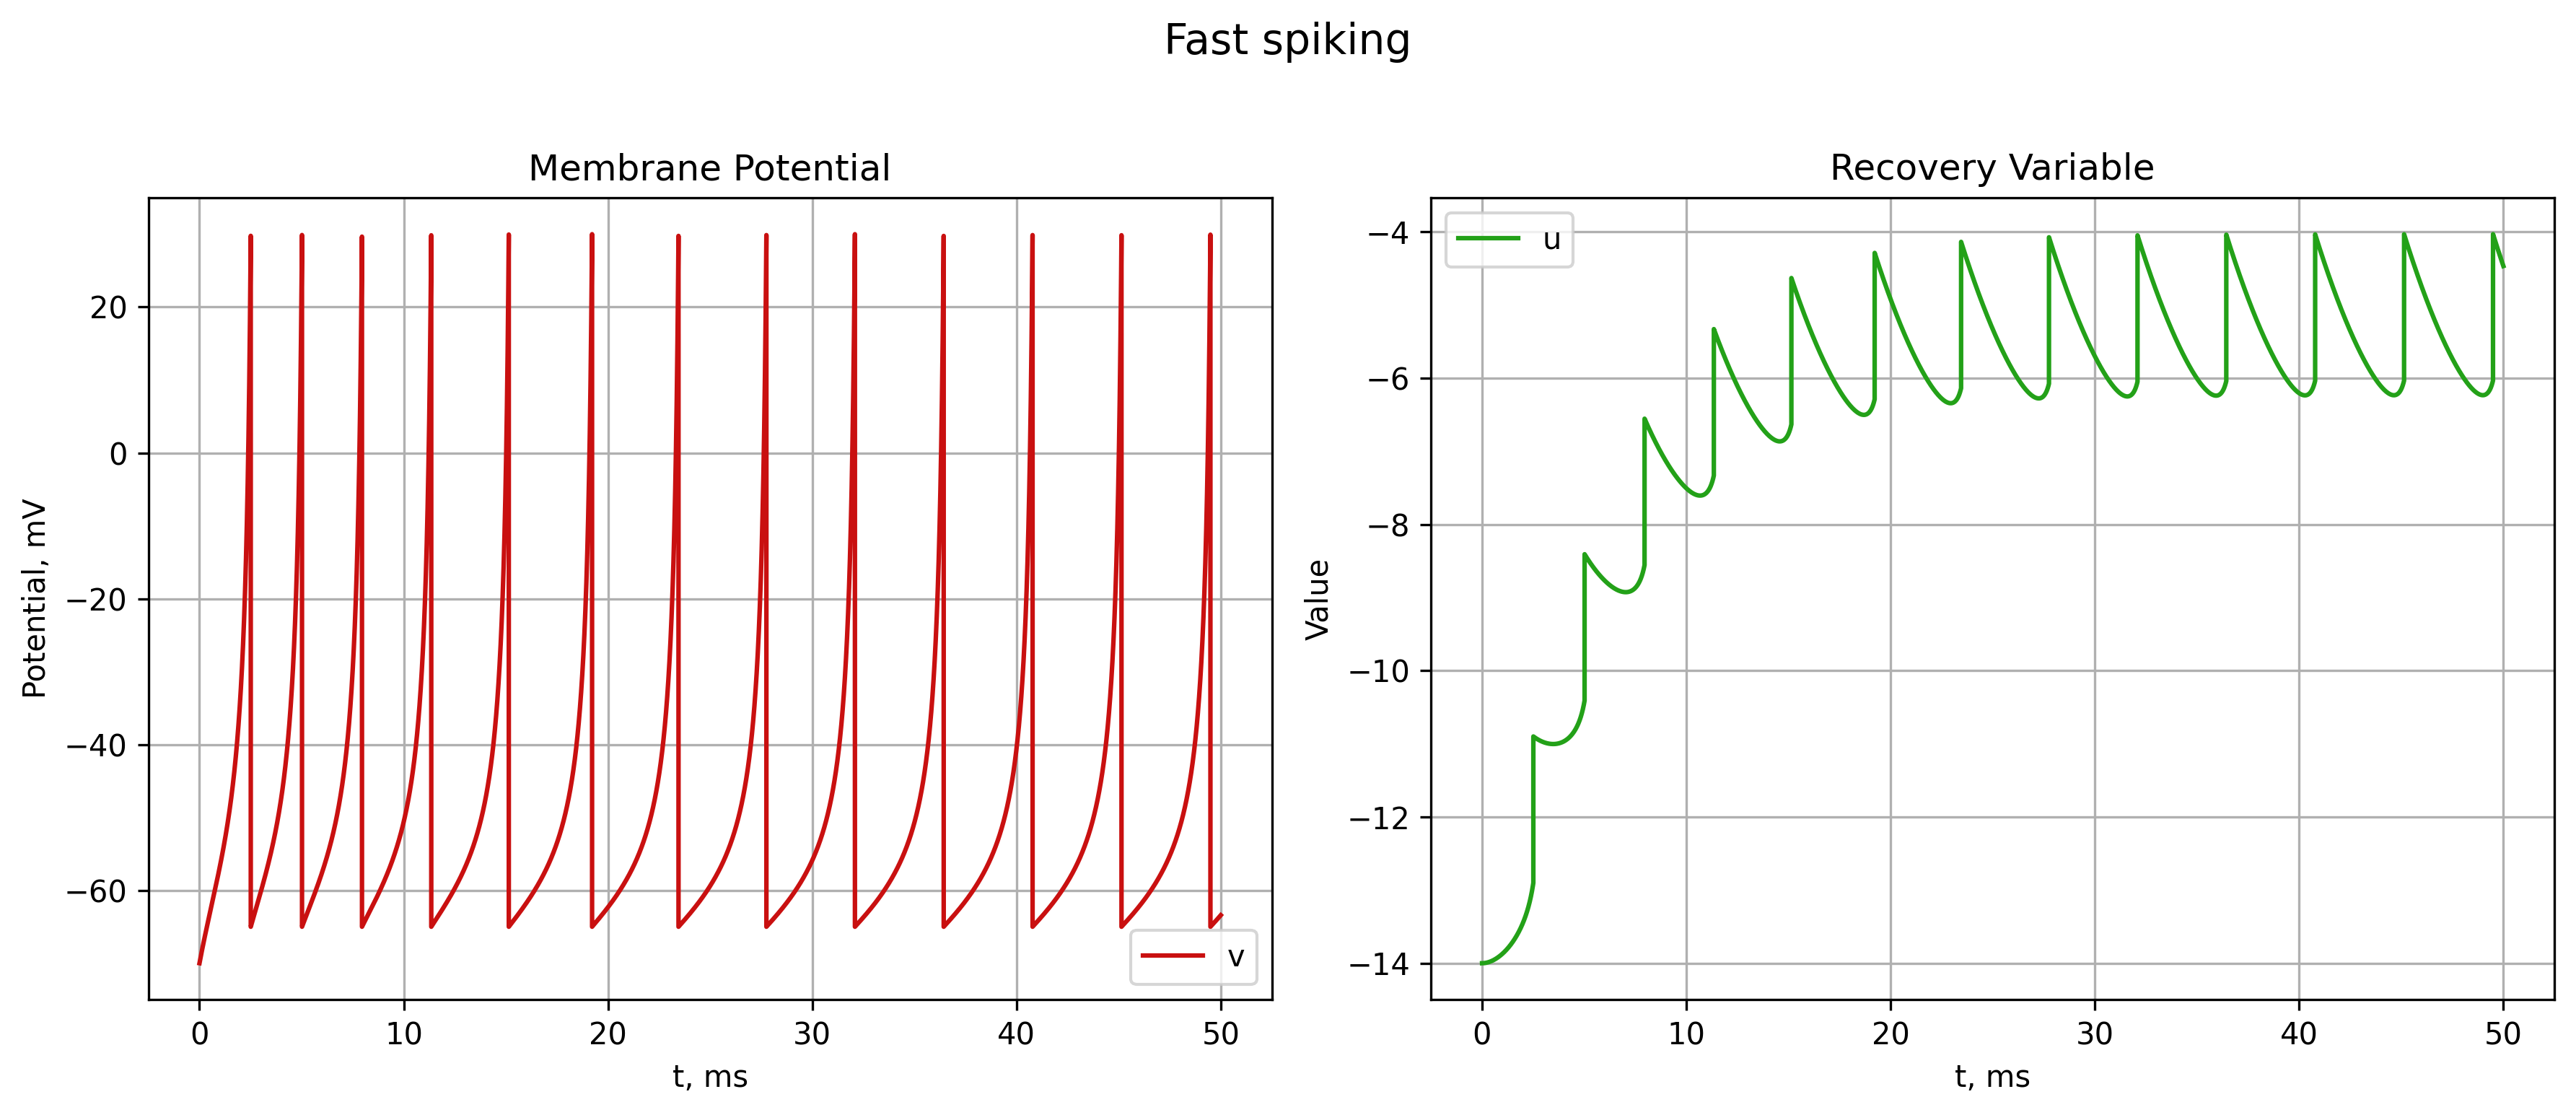
\includegraphics[width=1\linewidth]{pic/fast_spiking.png}}
\caption{Визуализация быстро-спайкового нейрона при $I=15$ нА.}
\label{1_fs}
\end{figure}

\begin{figure}[h]
	\center{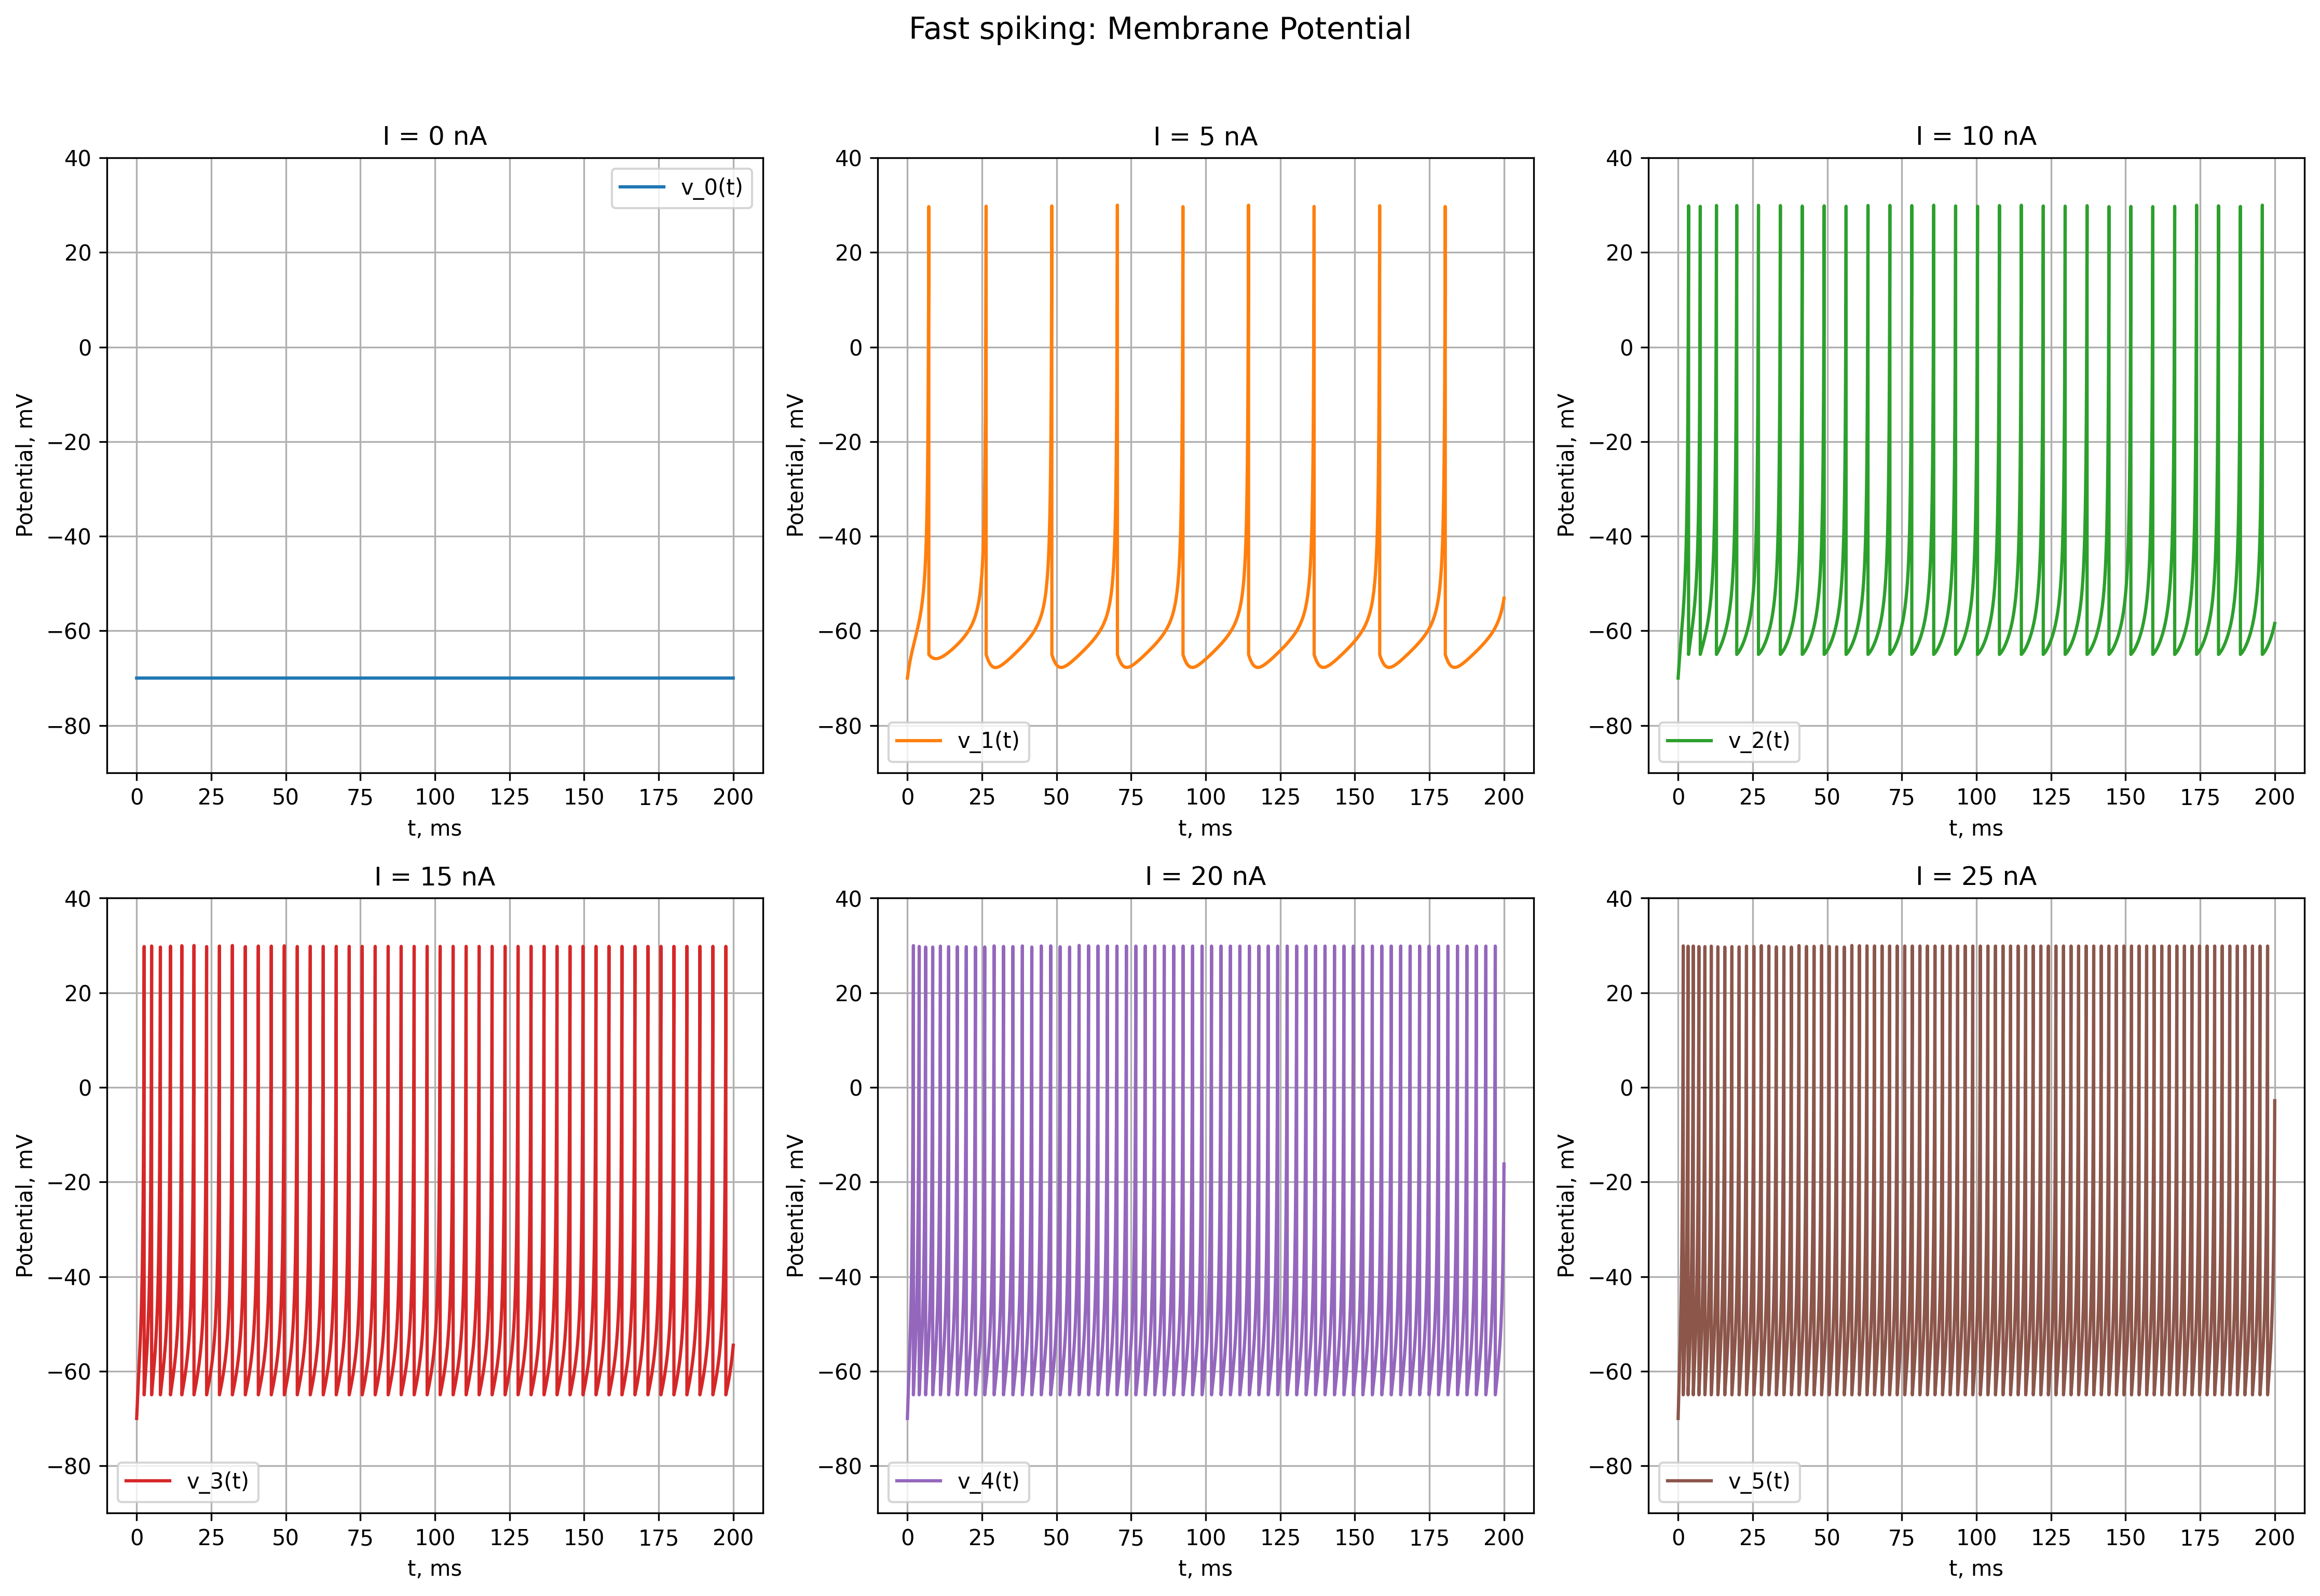
\includegraphics[width=1\linewidth]{pic/fs_different_I_potentials.png}}
	\caption{Визуализация $v(t)$ быстро-спайкового нейрона для разных значений $I$.}
	\label{fs_different_I_potentials}
\end{figure}

\begin{figure}[h]
	\center{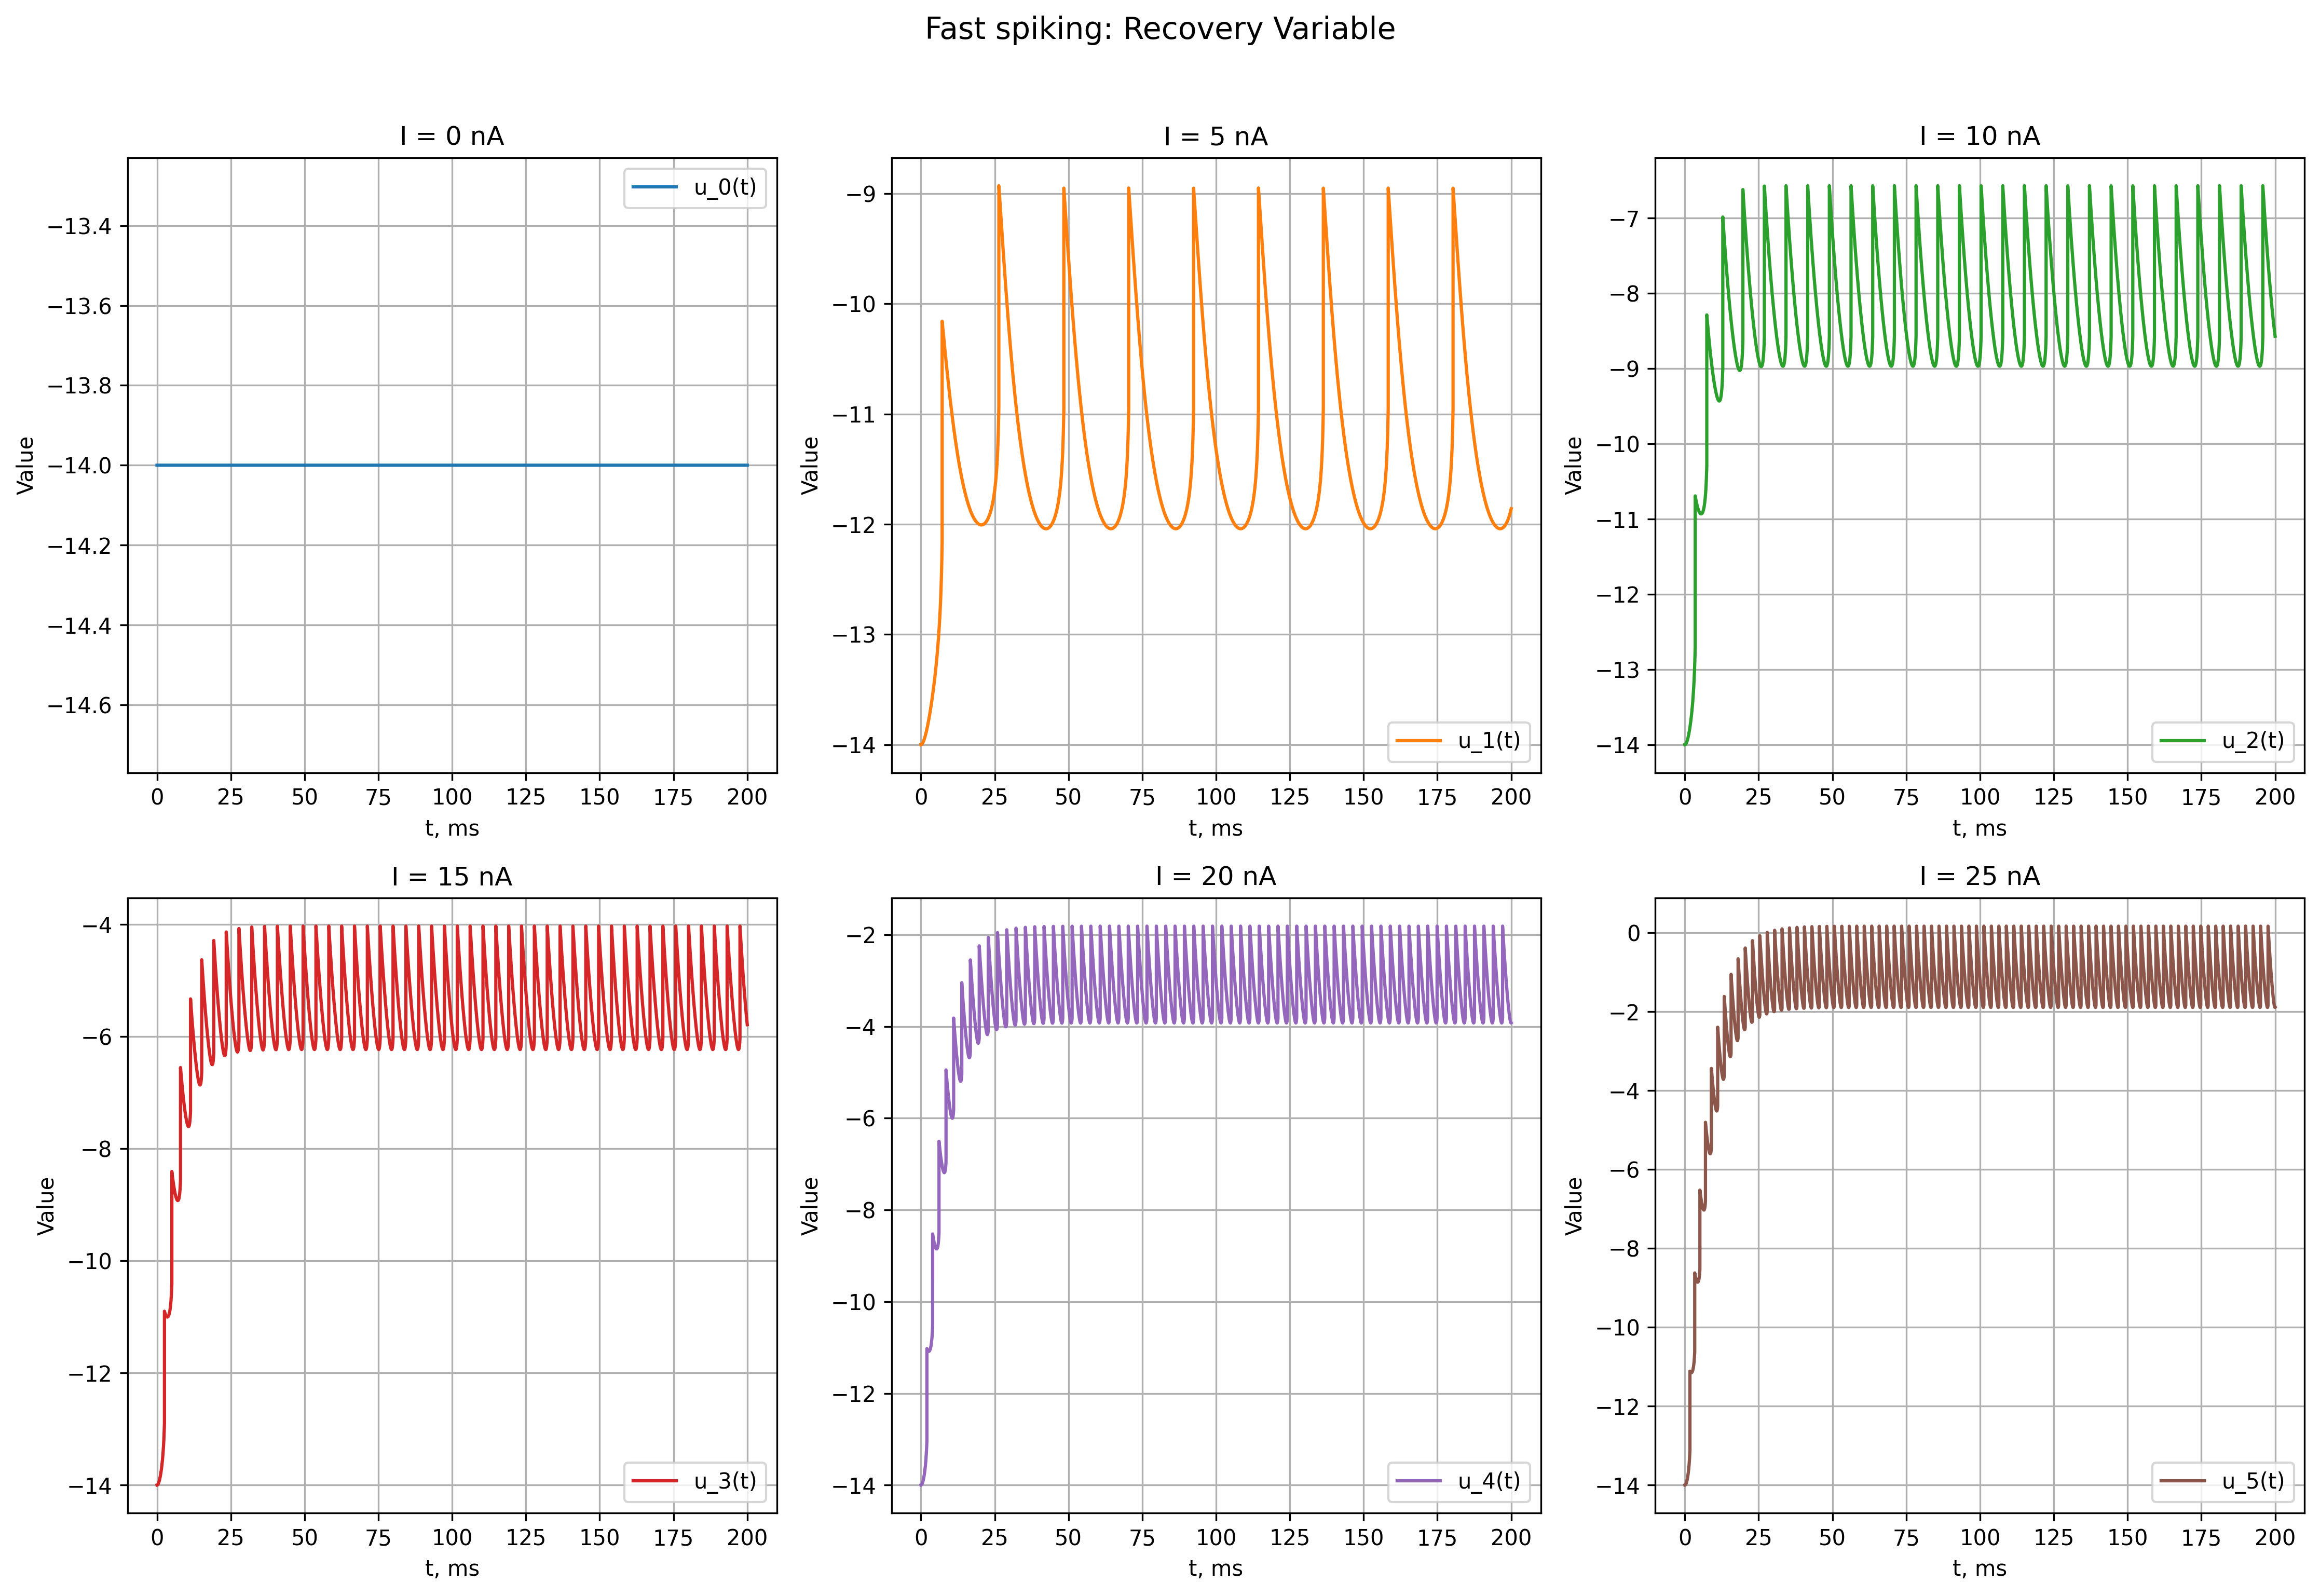
\includegraphics[width=1\linewidth]{pic/fs_different_I_recovery.png}}
	\caption{Визуализация $u(t)$ быстро-спайкового нейрона для разных значений $I$.}
	\label{fs_different_I_recovery}
\end{figure}

\begin{figure}[h]
\center{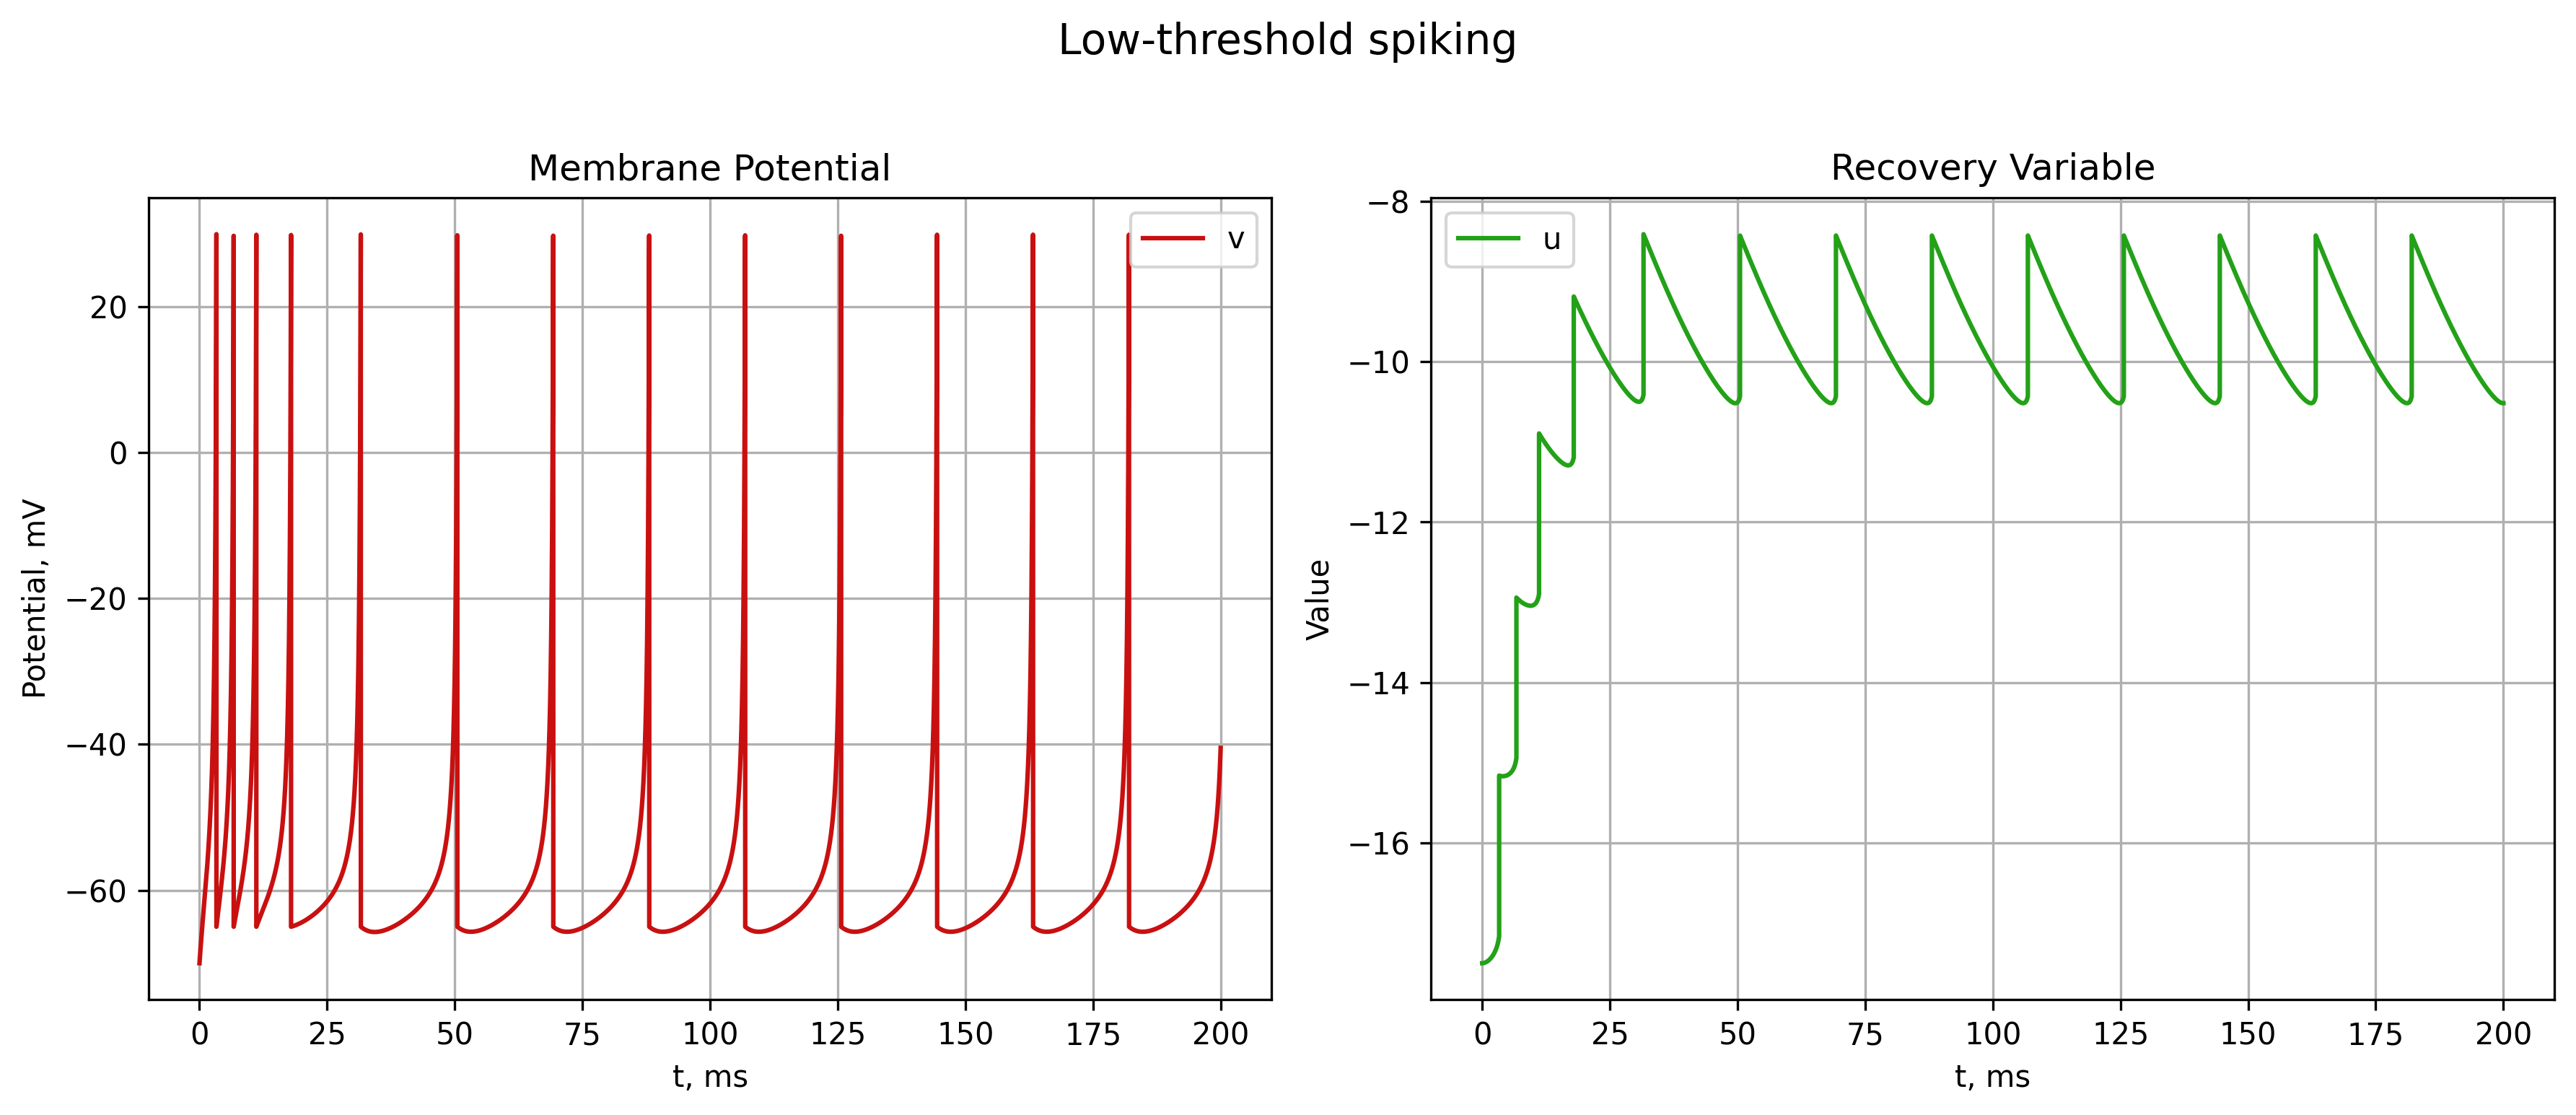
\includegraphics[width=1\linewidth]{pic/low_threshold_spiking.png}}
\caption{Визуализация низкопорогового спайкового нейрона при $I=7$ нА.}
\label{1_lts}
\end{figure}

\begin{figure}[h]
	\center{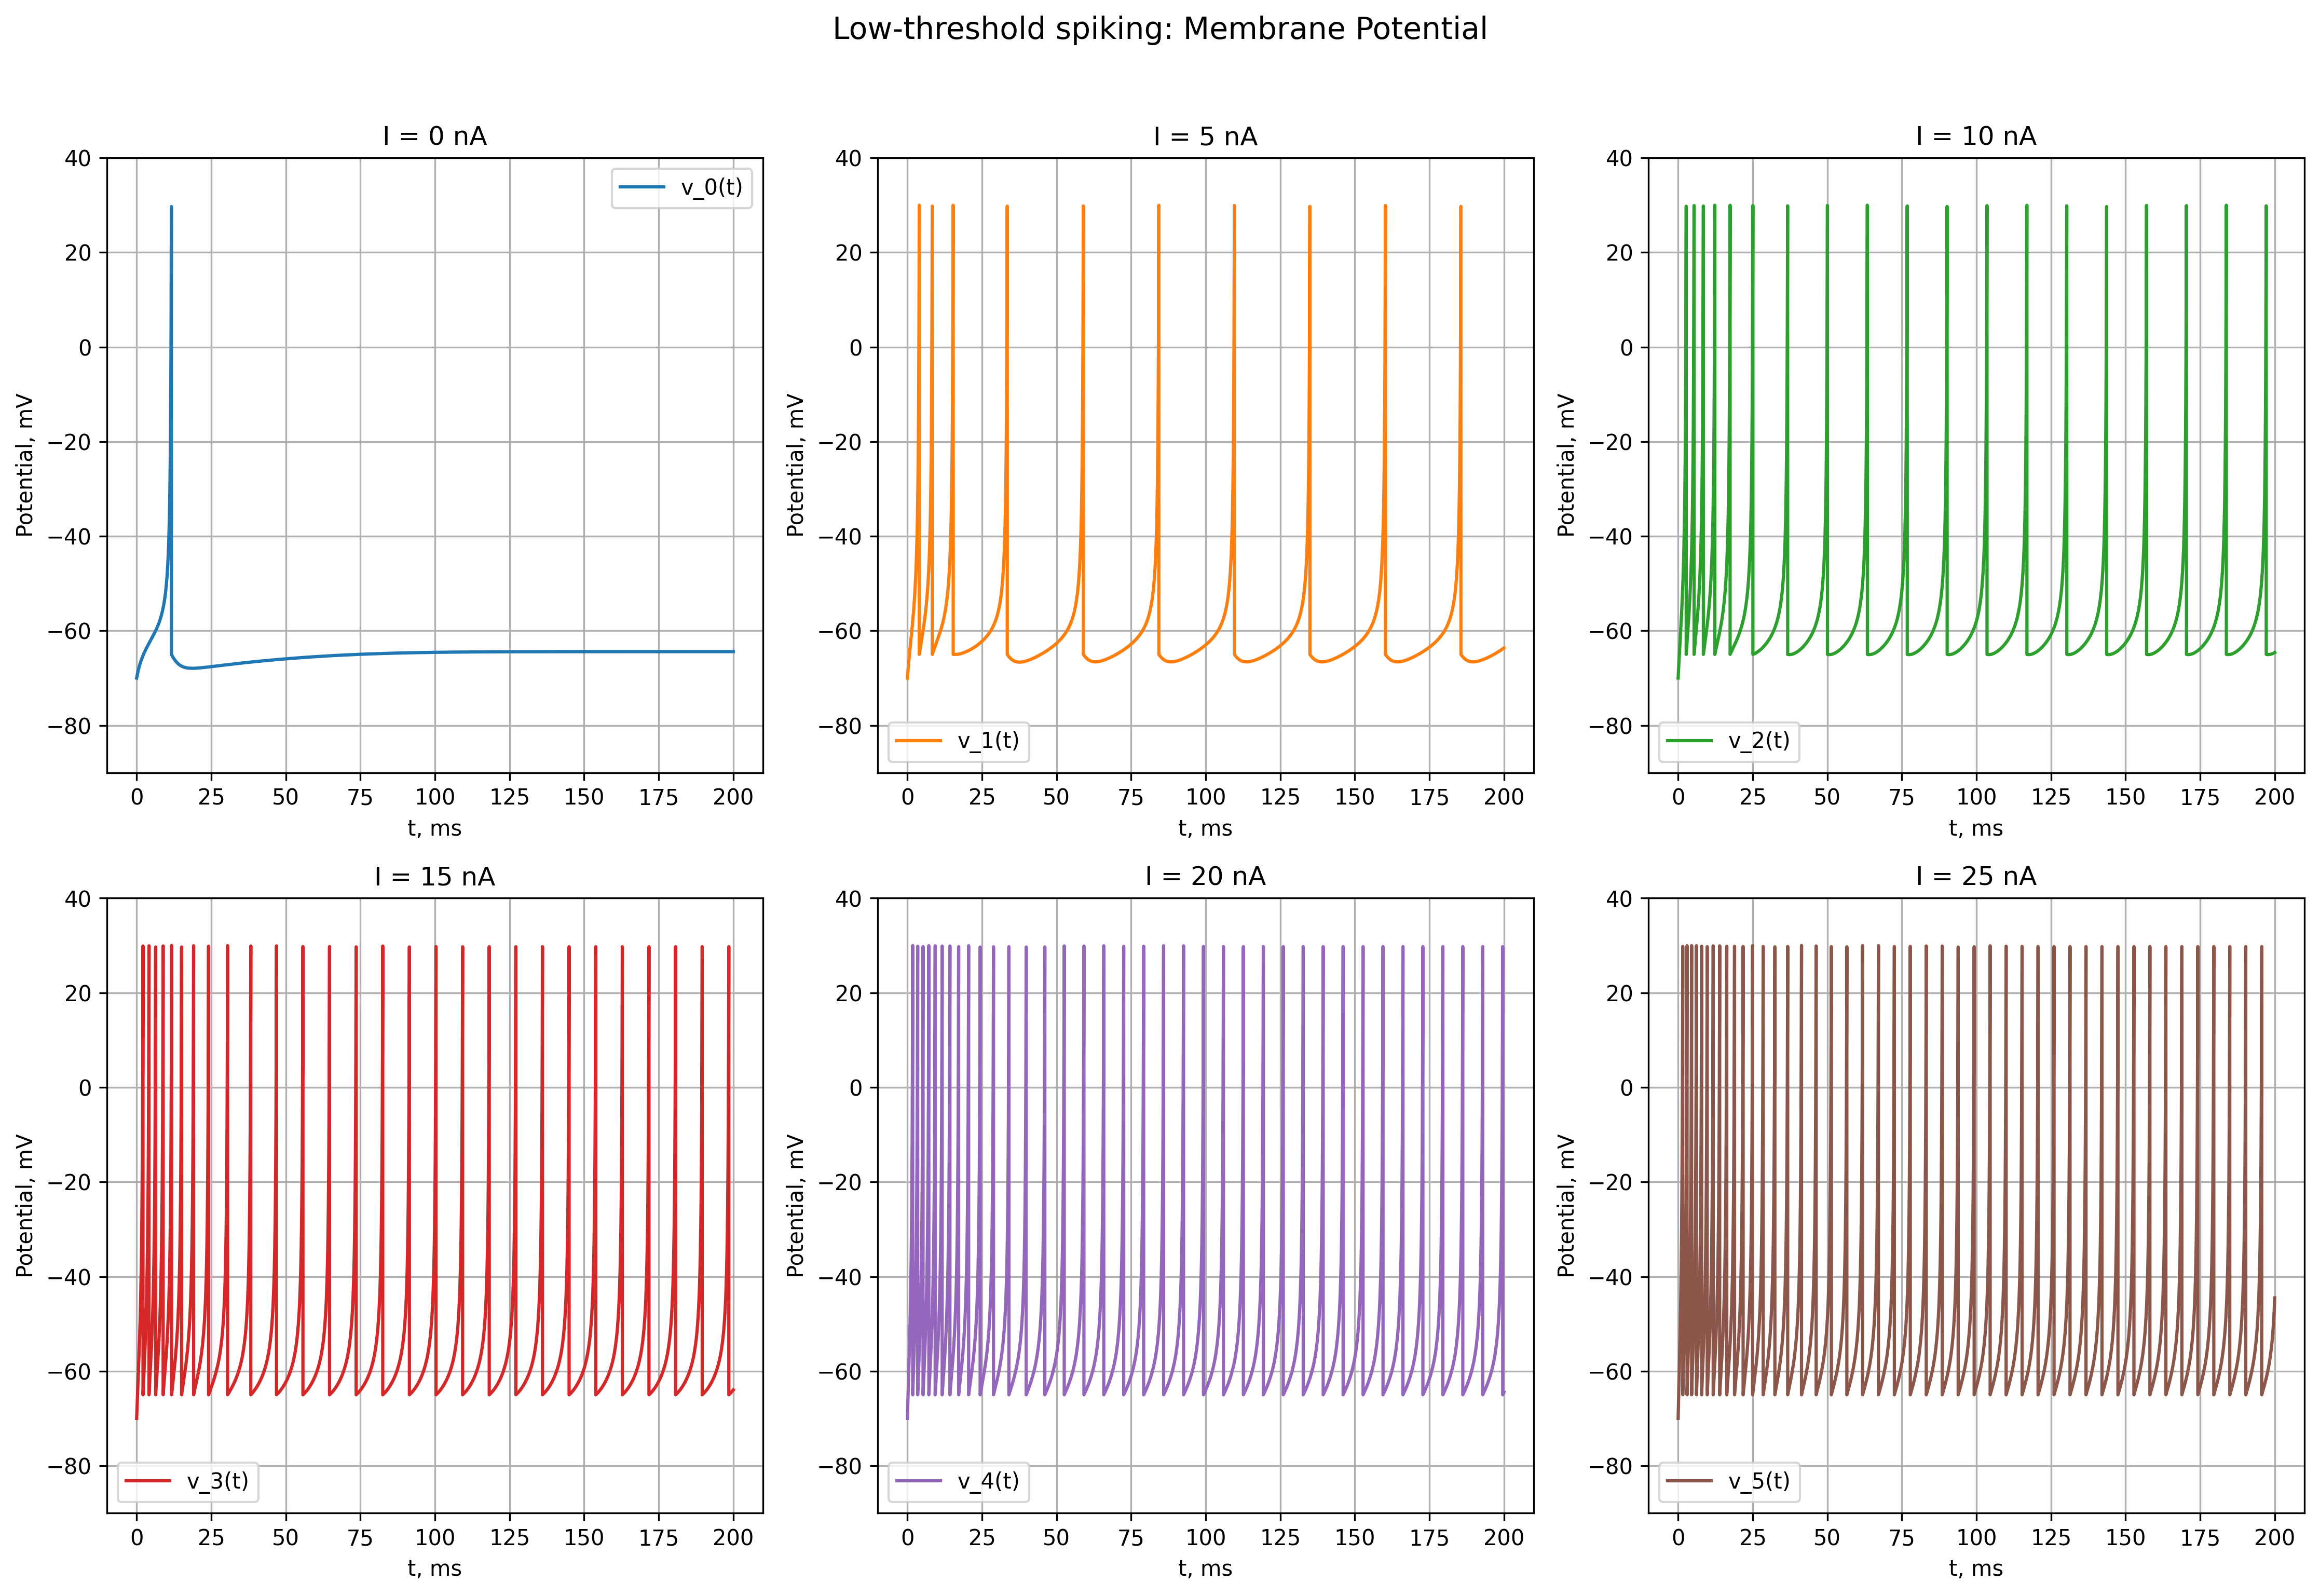
\includegraphics[width=1\linewidth]{pic/lts_different_I_potentials.png}}
	\caption{Визуализация $v(t)$ низкопорогового спайкового нейрона для разных значений $I$.}
	\label{lts_different_I_potentials}
\end{figure}

\begin{figure}[h]
	\center{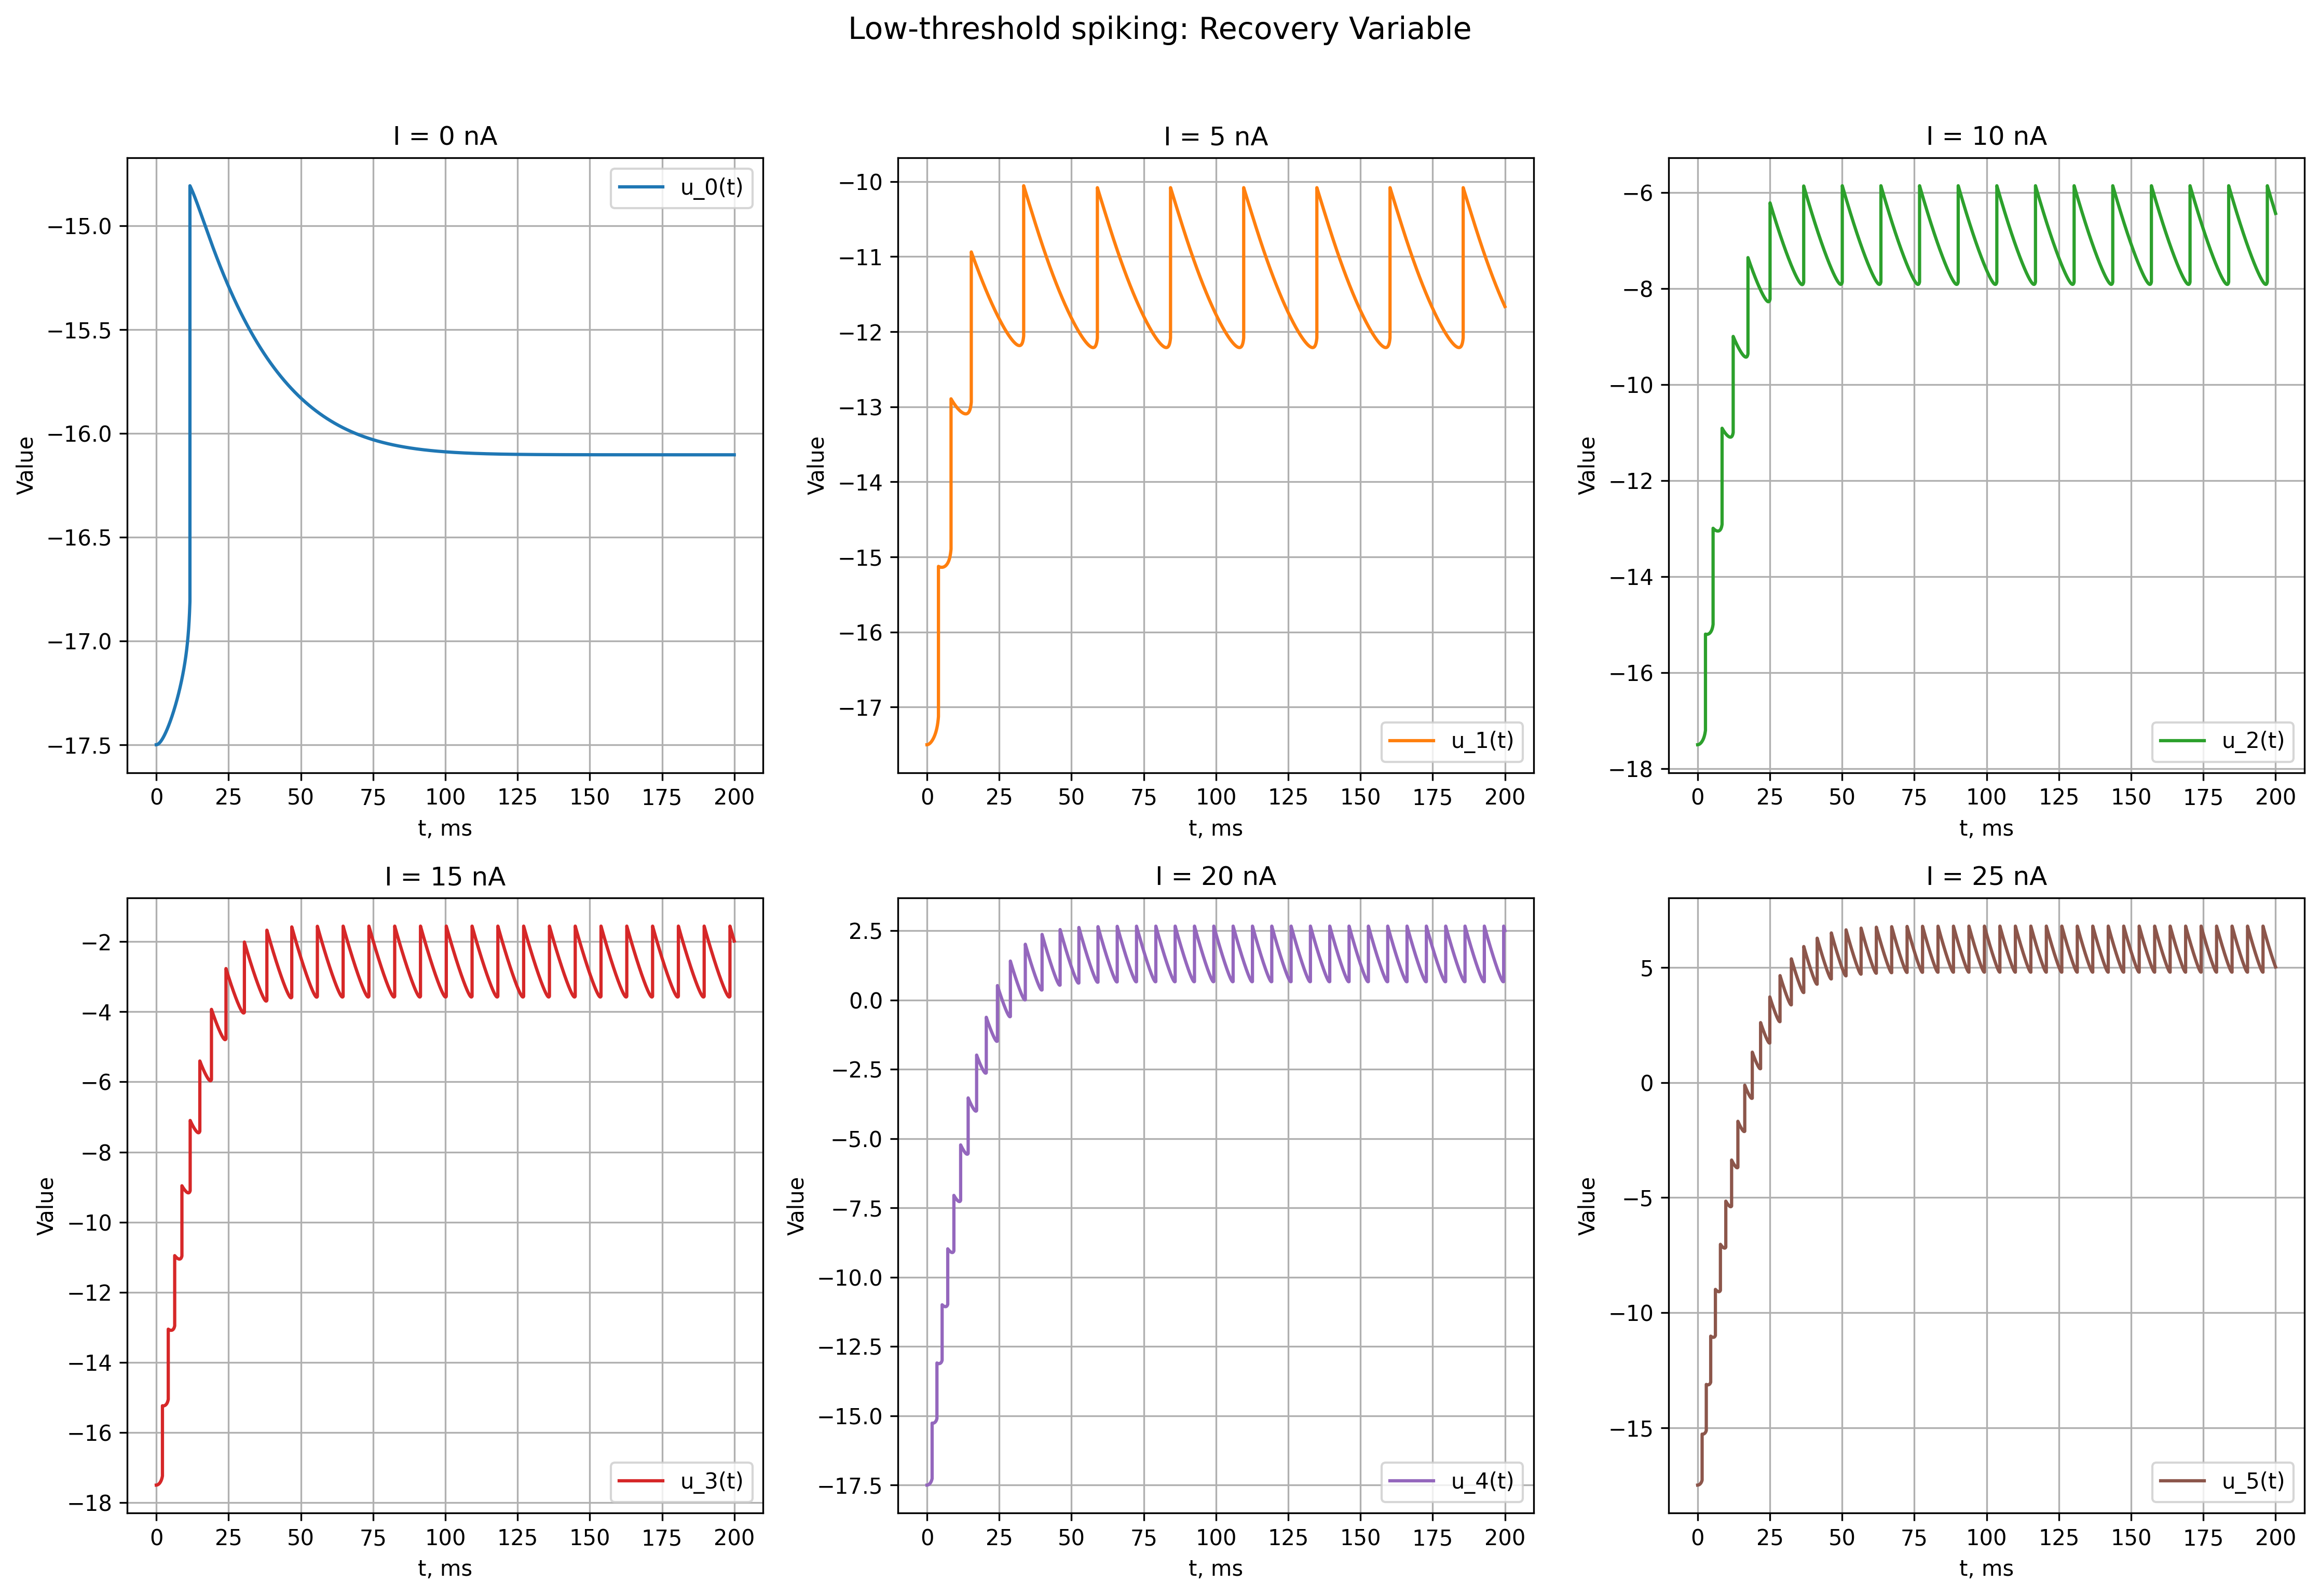
\includegraphics[width=1\linewidth]{pic/lts_different_I_recovery.png}}
	\caption{Визуализация $u(t)$ низкопорогового спайкового нейрона для разных значений $I$.}
	\label{lts_different_I_recovery}
\end{figure}

\begin{figure}[h]
\center{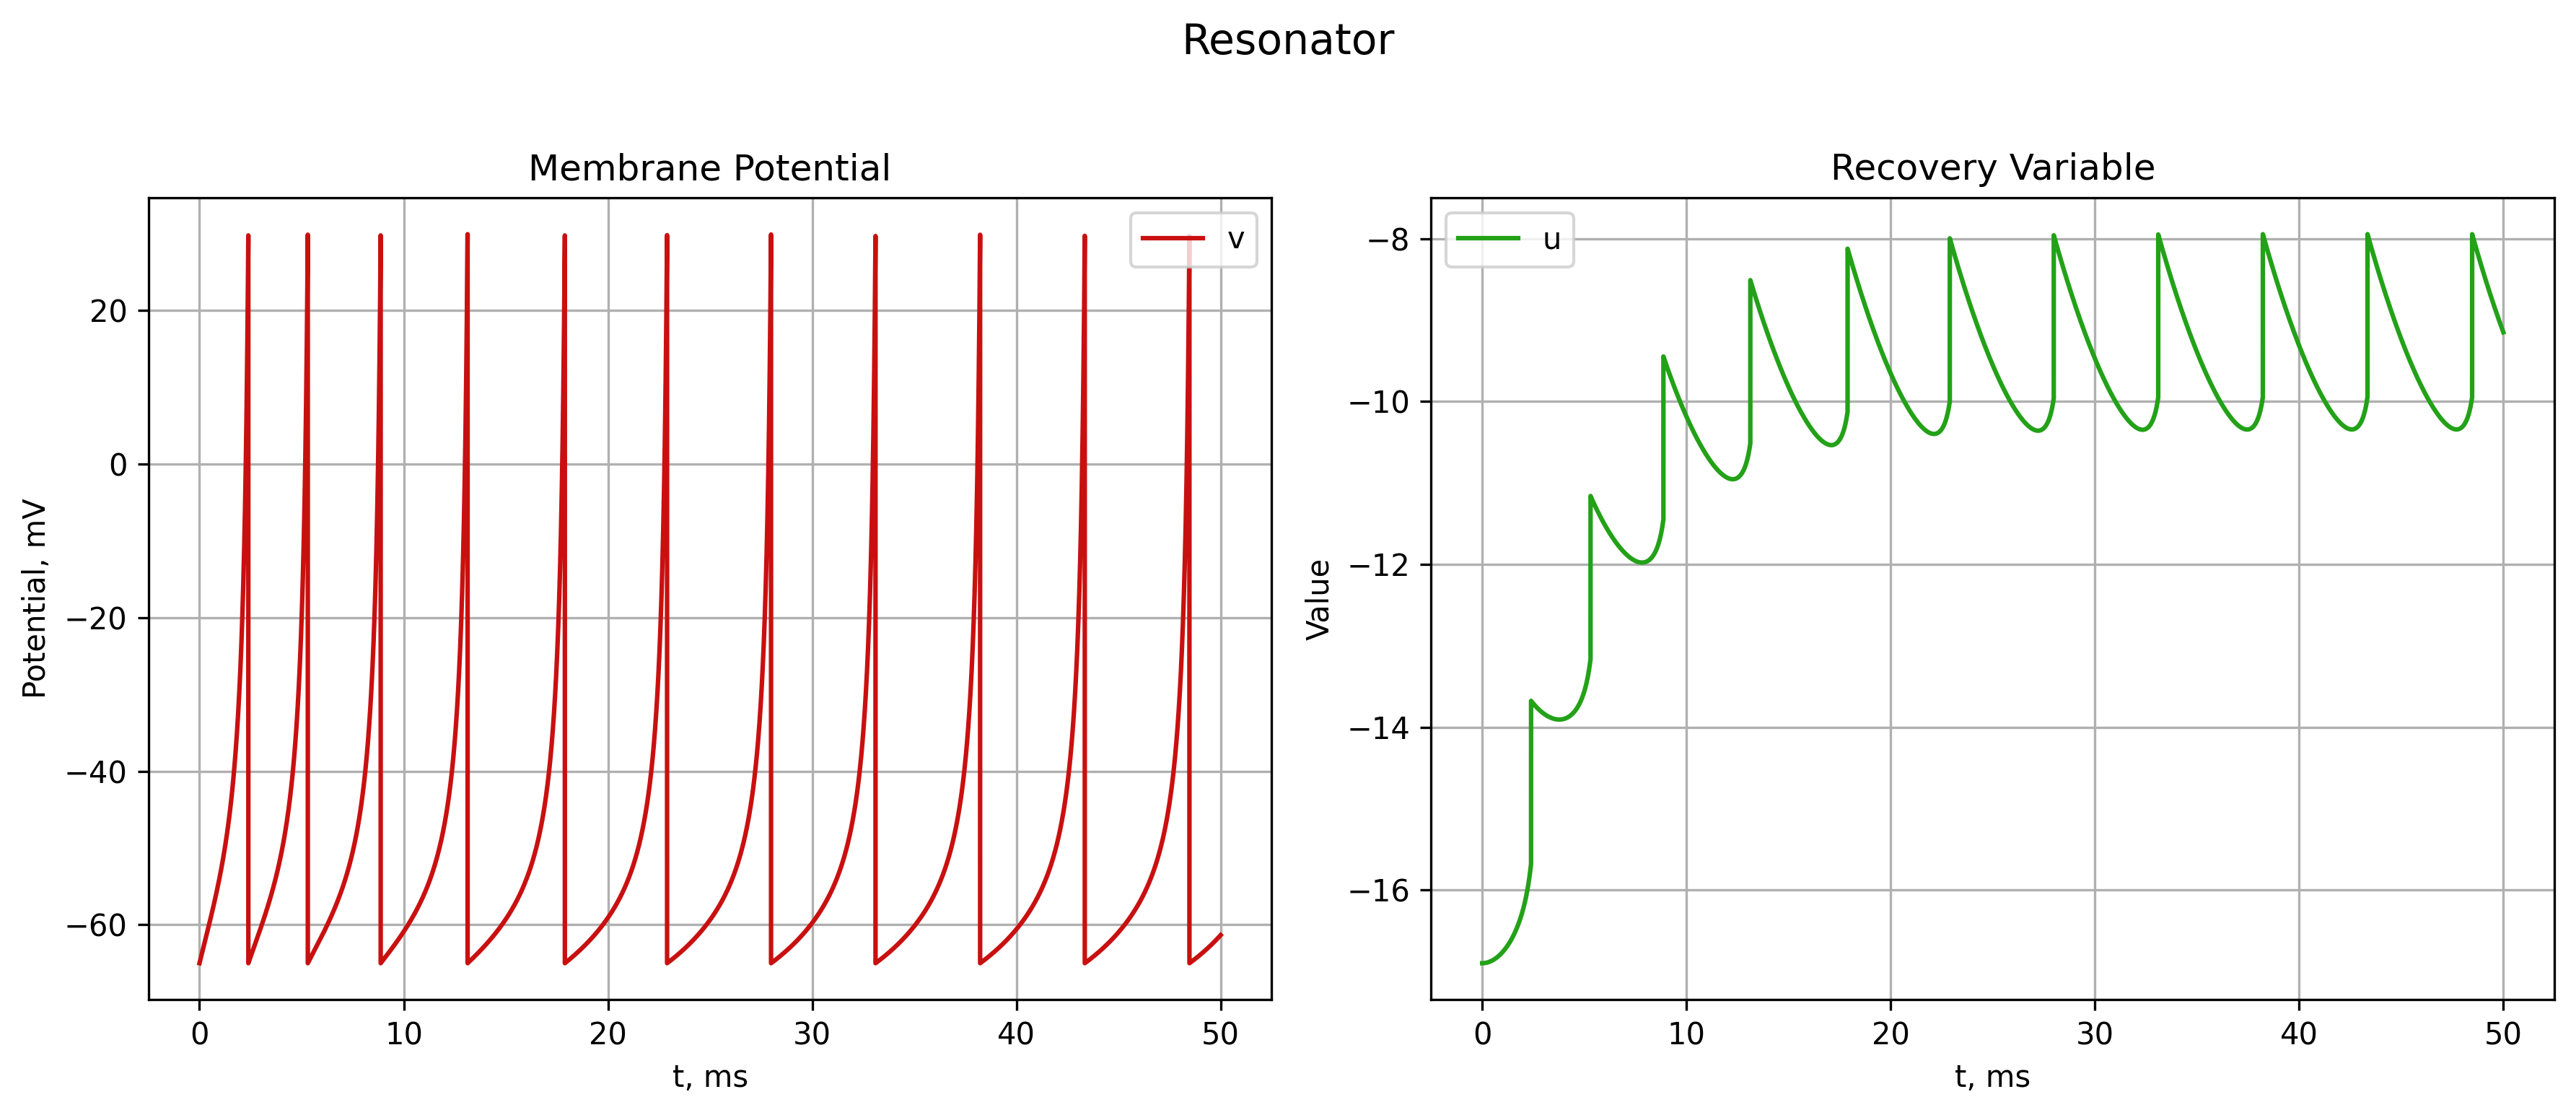
\includegraphics[width=1\linewidth]{pic/resonator_spiking.png}}
\caption{Визуализация резиллерно-спайкового нейрона при $I=10$ нА.}
\label{1_rz}
\end{figure}

\begin{figure}[h]
	\center{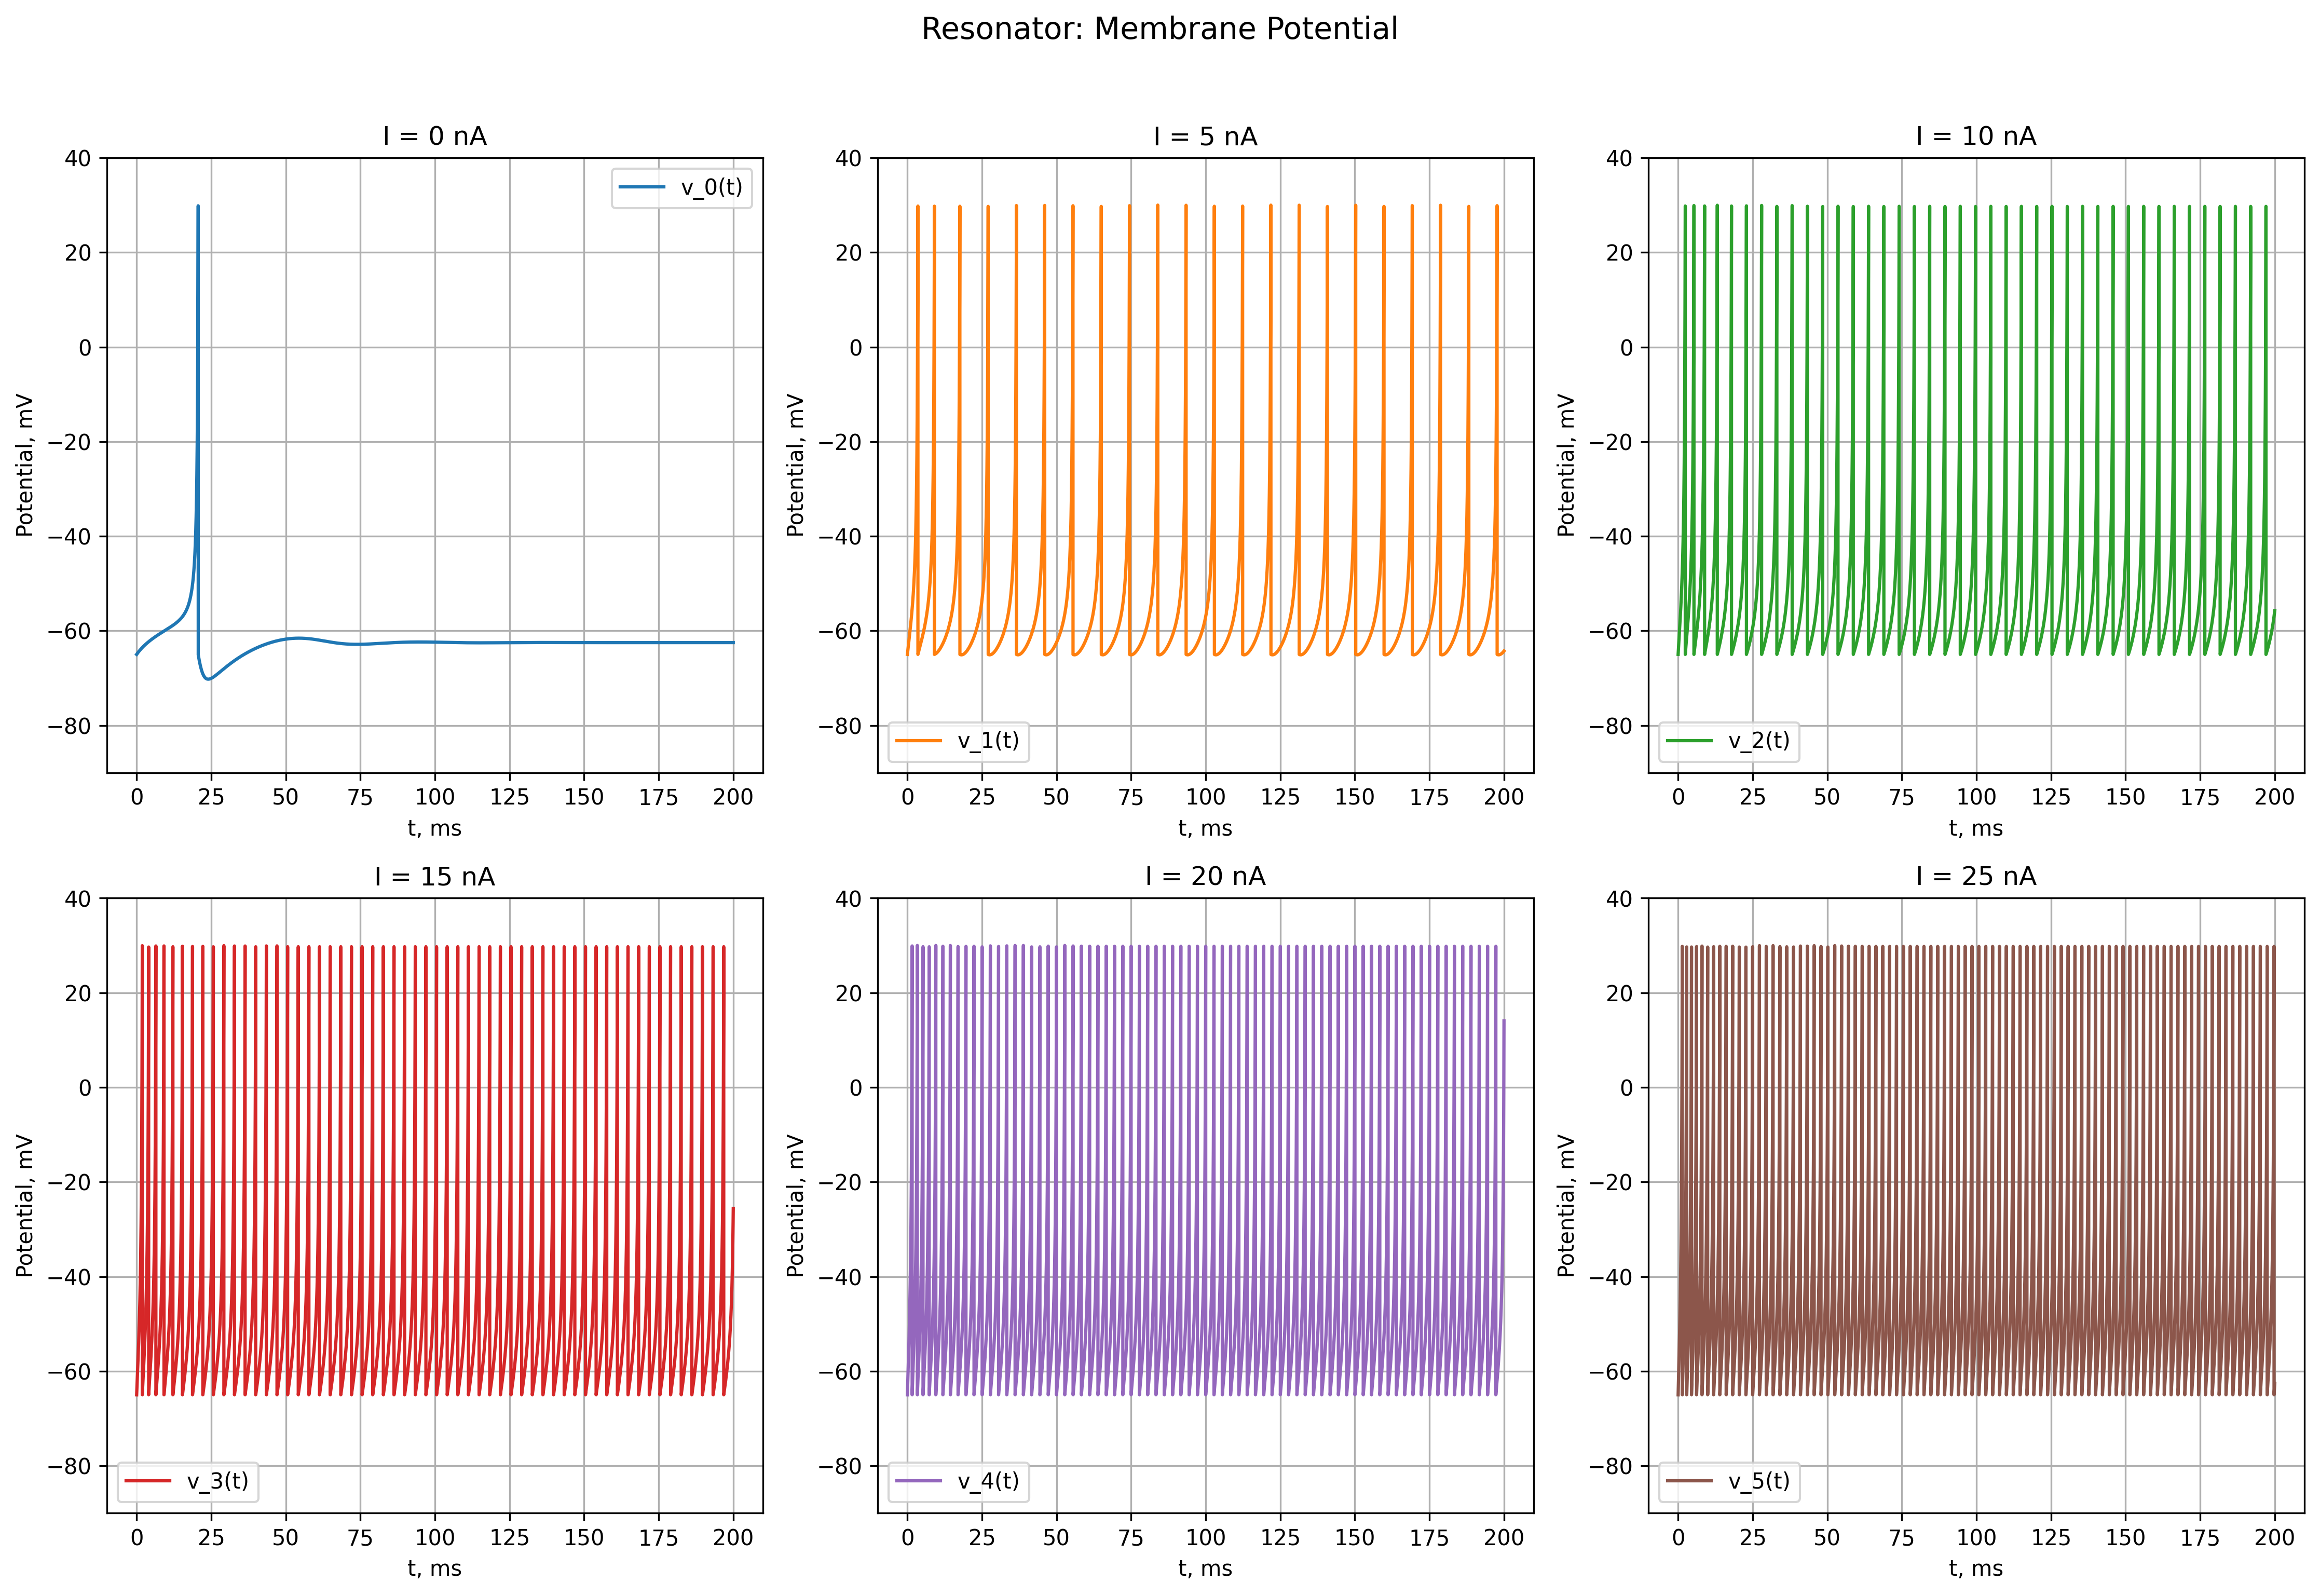
\includegraphics[width=1\linewidth]{pic/rz_different_I_potentials.png}}
	\caption{Визуализация $v(t)$ резиллерно-спайкового нейрона для разных значений $I$.}
	\label{rz_different_I_potentials}
\end{figure}

\begin{figure}[h]
	\center{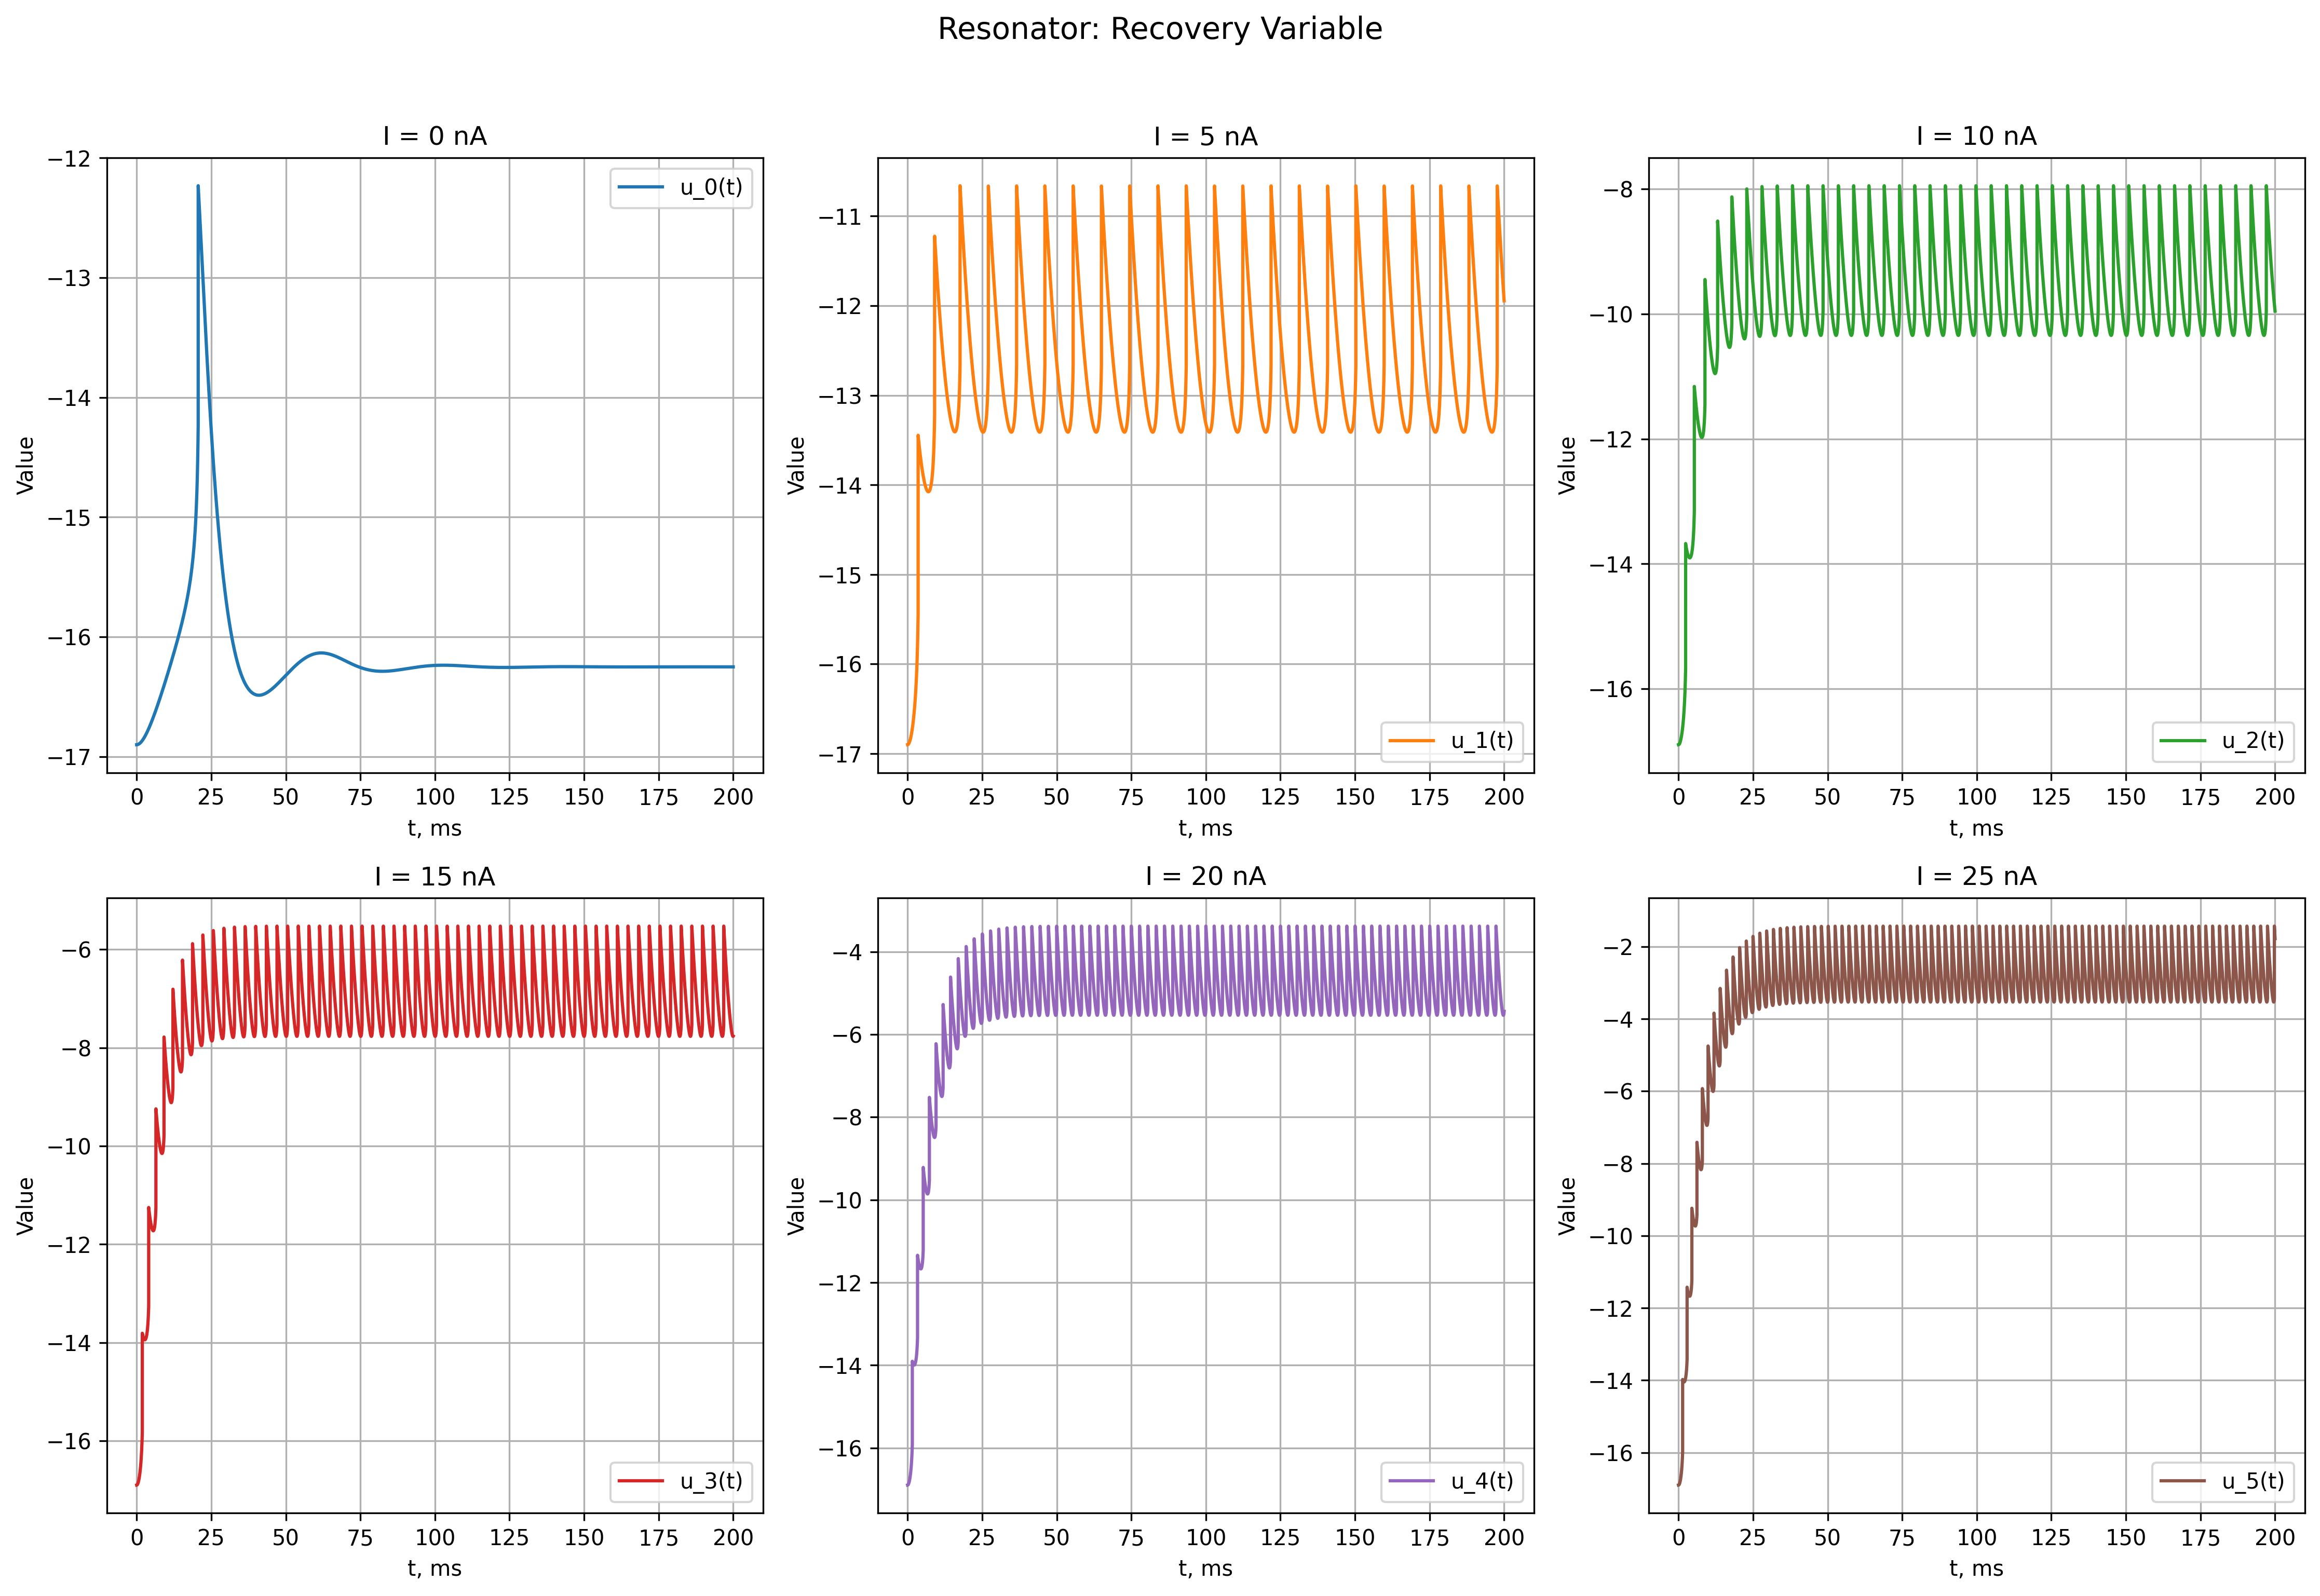
\includegraphics[width=1\linewidth]{pic/rz_different_I_recovery.png}}
	\caption{Визуализация $u(t)$ резиллерно-спайкового нейрона для разных значений $I$.}
	\label{rz_different_I_recovery}
\end{figure}

\begin{figure}[h]
\center{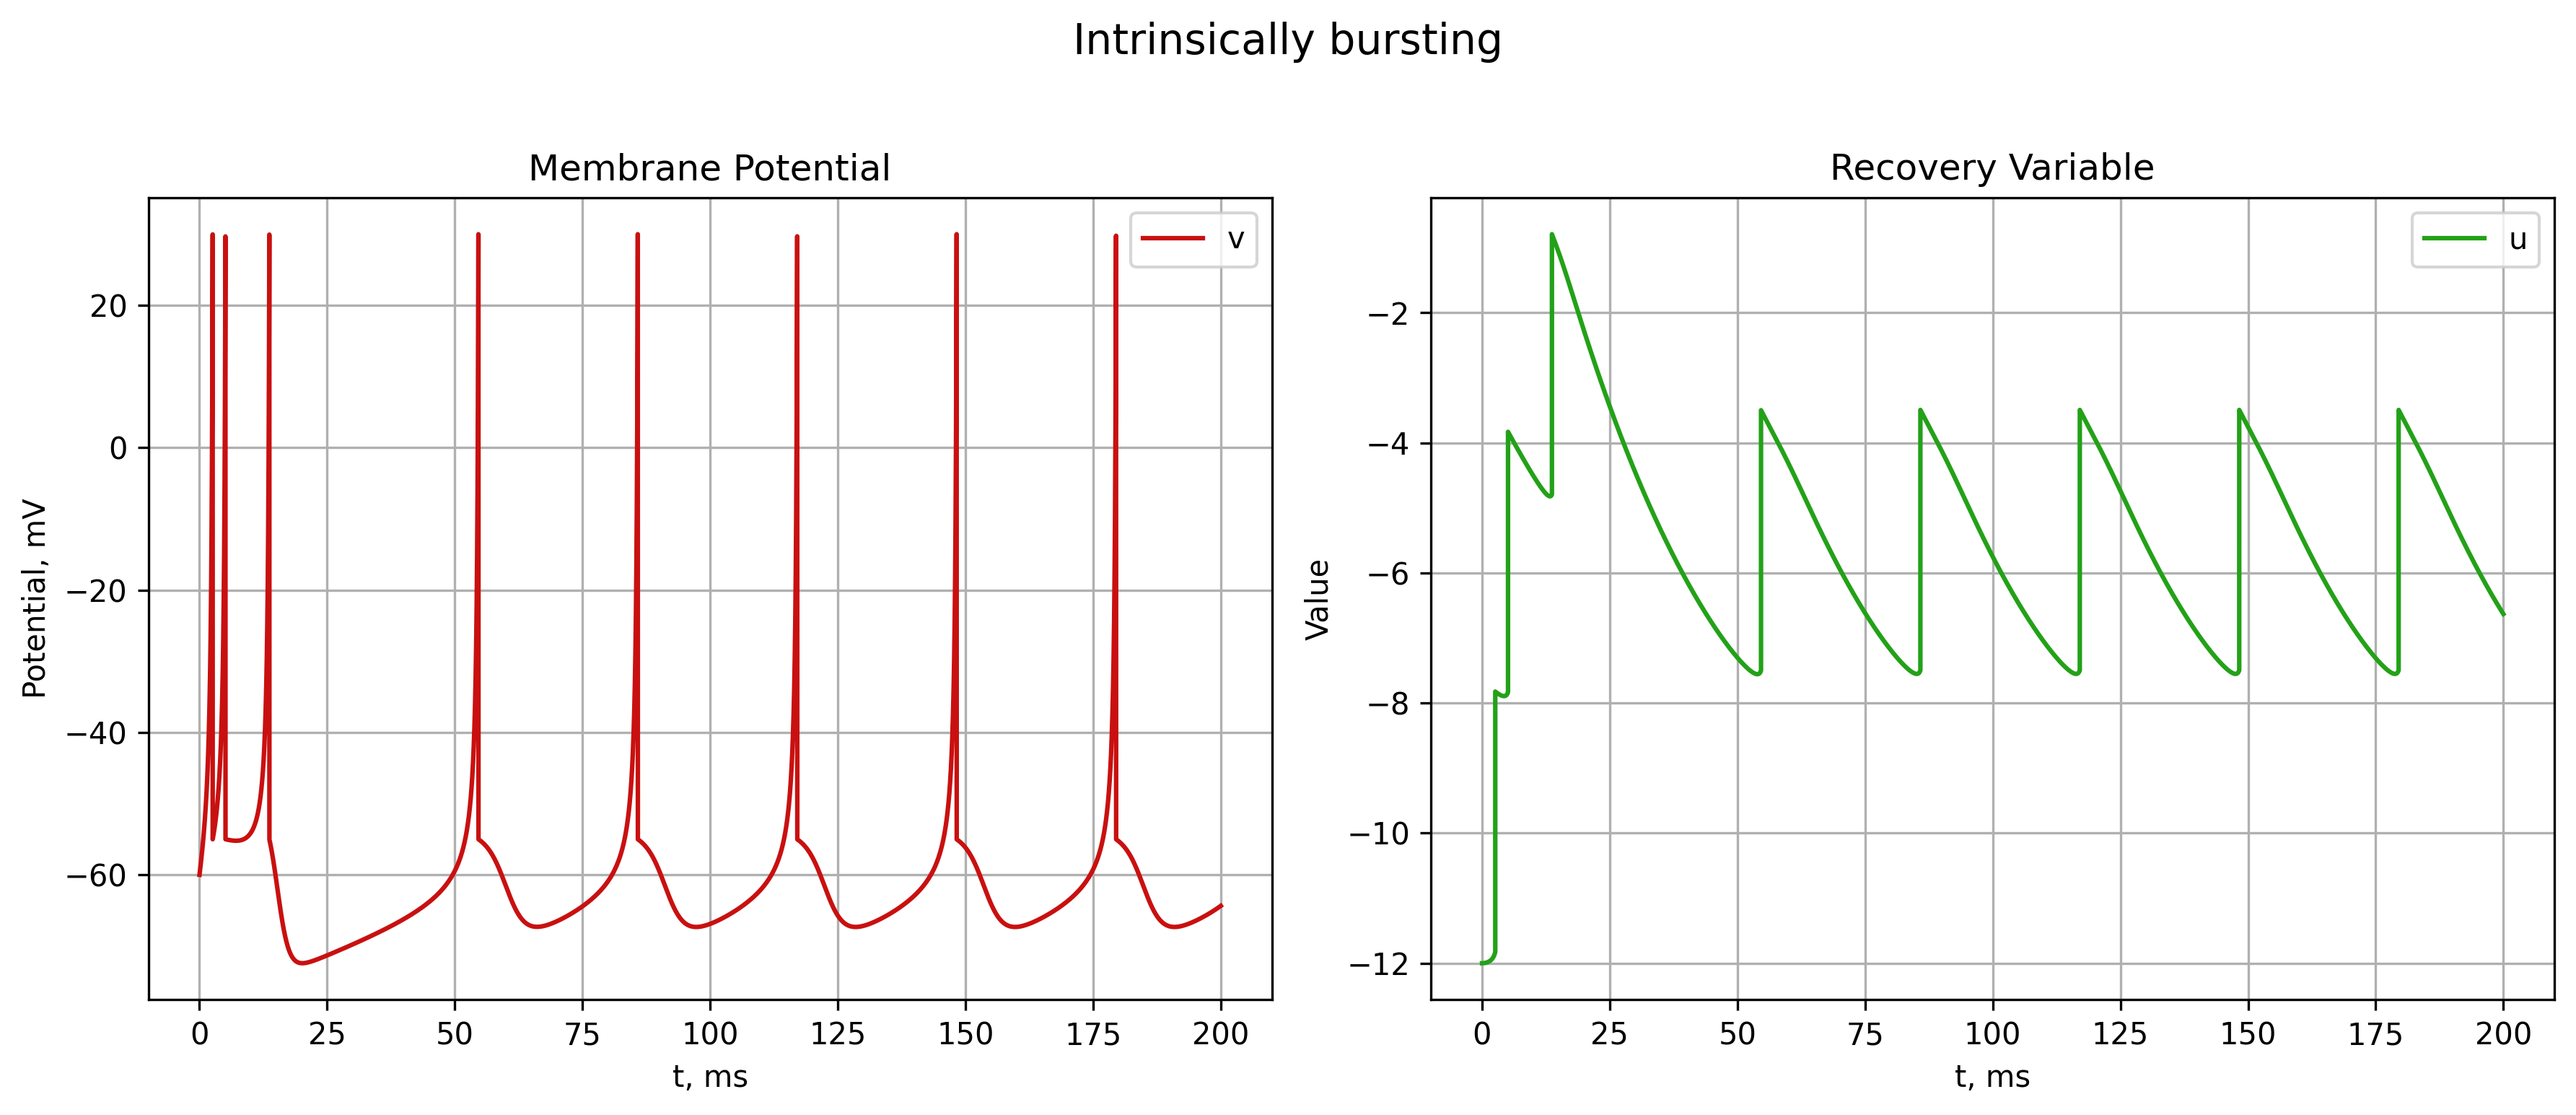
\includegraphics[width=1\linewidth]{pic/intrinsically_bursting.png}}
\caption{Визуализация интринсивно-всплескового нейрона при $I=10$ нА.}
\label{1_ib}
\end{figure}

\begin{figure}[h]
	\center{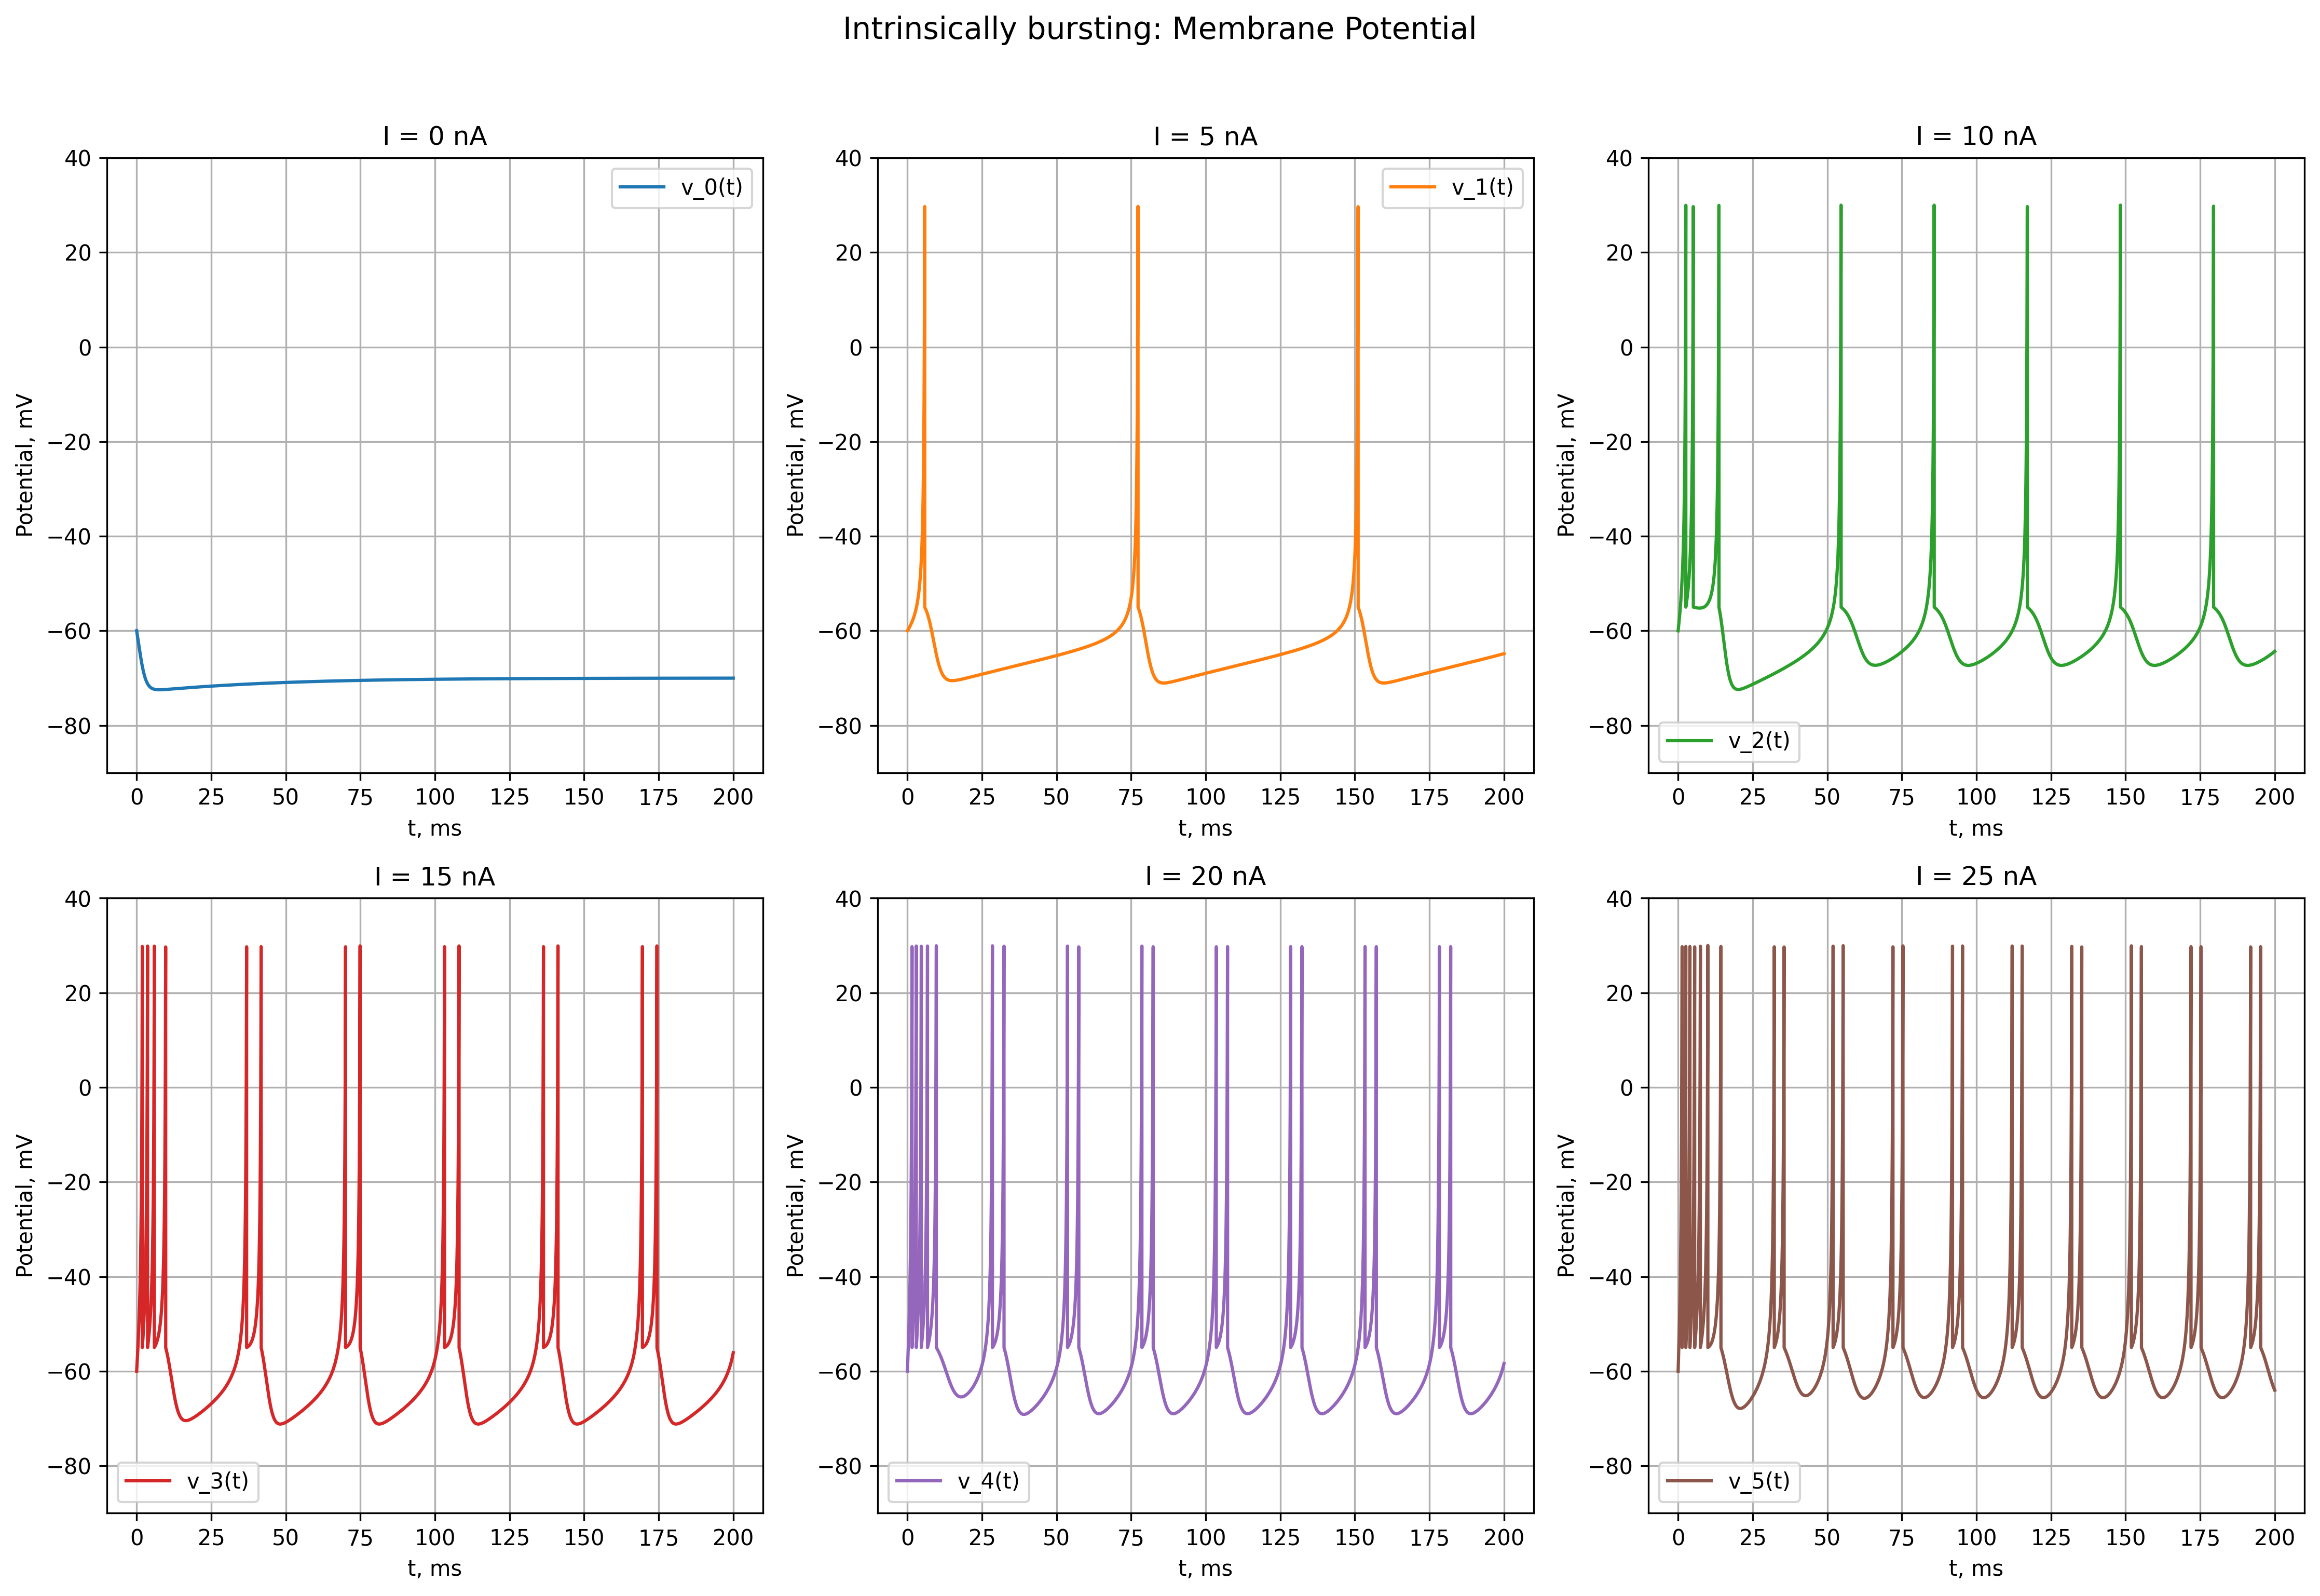
\includegraphics[width=1\linewidth]{pic/ib_different_I_potentials.png}}
	\caption{Визуализация $v(t)$ интринсивно-всплескового нейрона для разных значений $I$.}
	\label{ib_different_I_potentials}
\end{figure}

\begin{figure}[h]
	\center{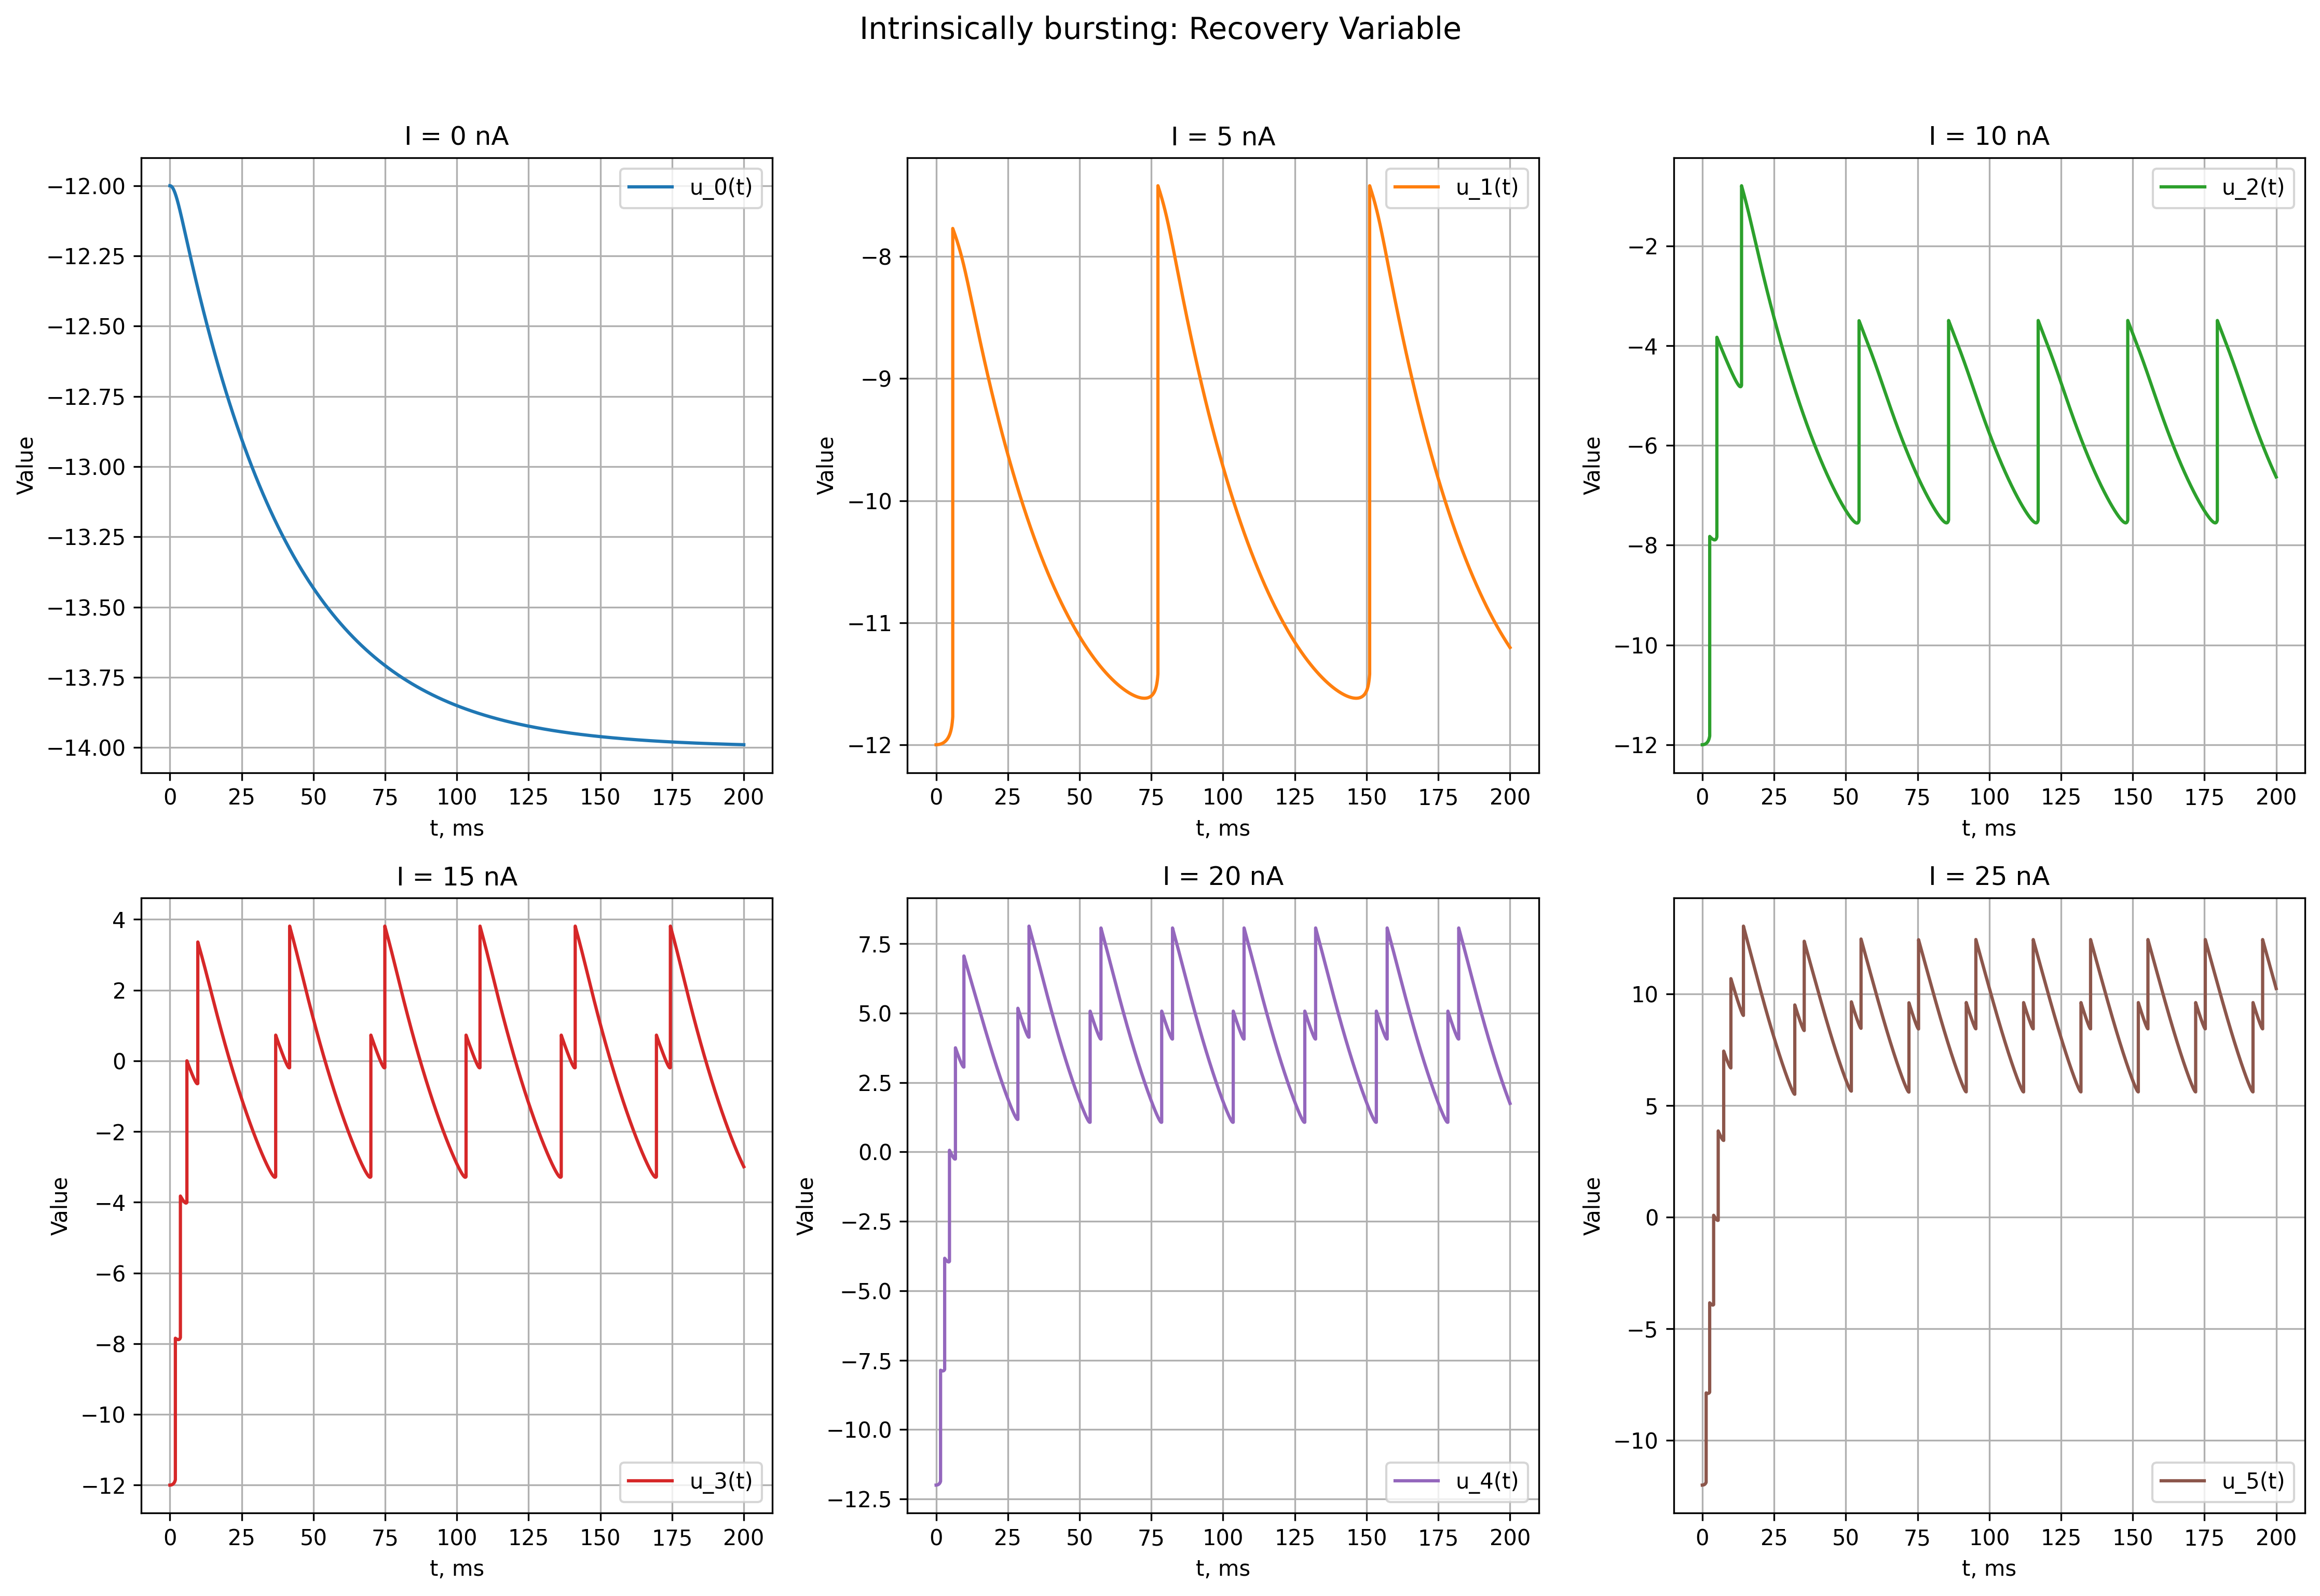
\includegraphics[width=1\linewidth]{pic/ib_different_I_recovery.png}}
	\caption{Визуализация $u(t)$ интринсивно-всплескового нейрона для разных значений $I$.}
	\label{ib_different_I_recovery}
\end{figure}

\begin{figure}[h]
\center{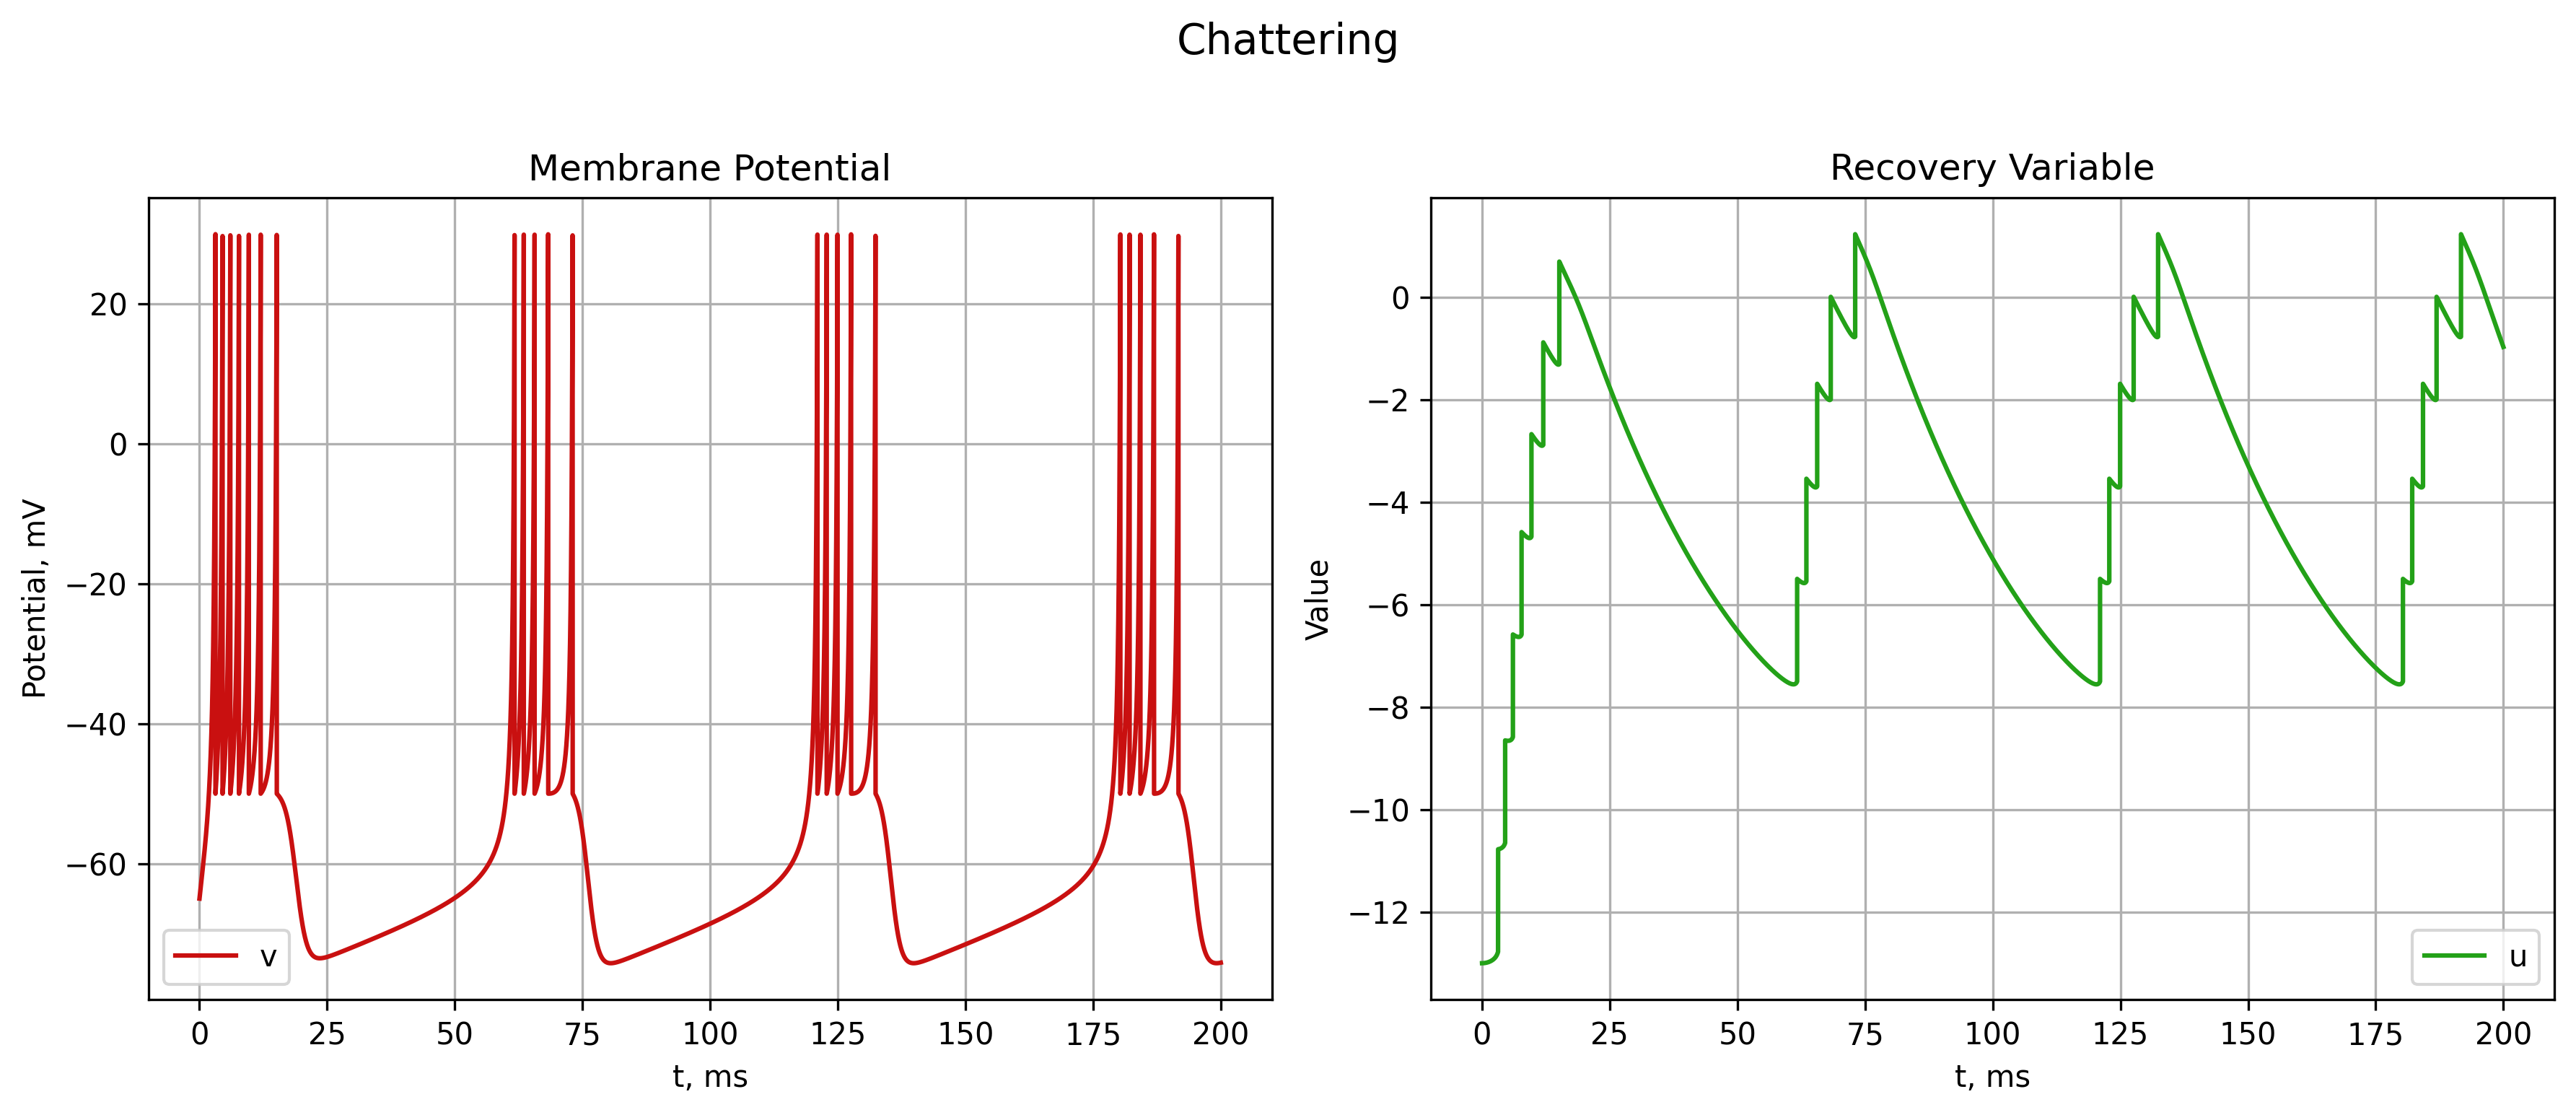
\includegraphics[width=1\linewidth]{pic/chattering.png}}
\caption{Визуализация частотного нейрона при $I=10$ нА.}
\label{1_ch}
\end{figure}

\begin{figure}[h]
	\center{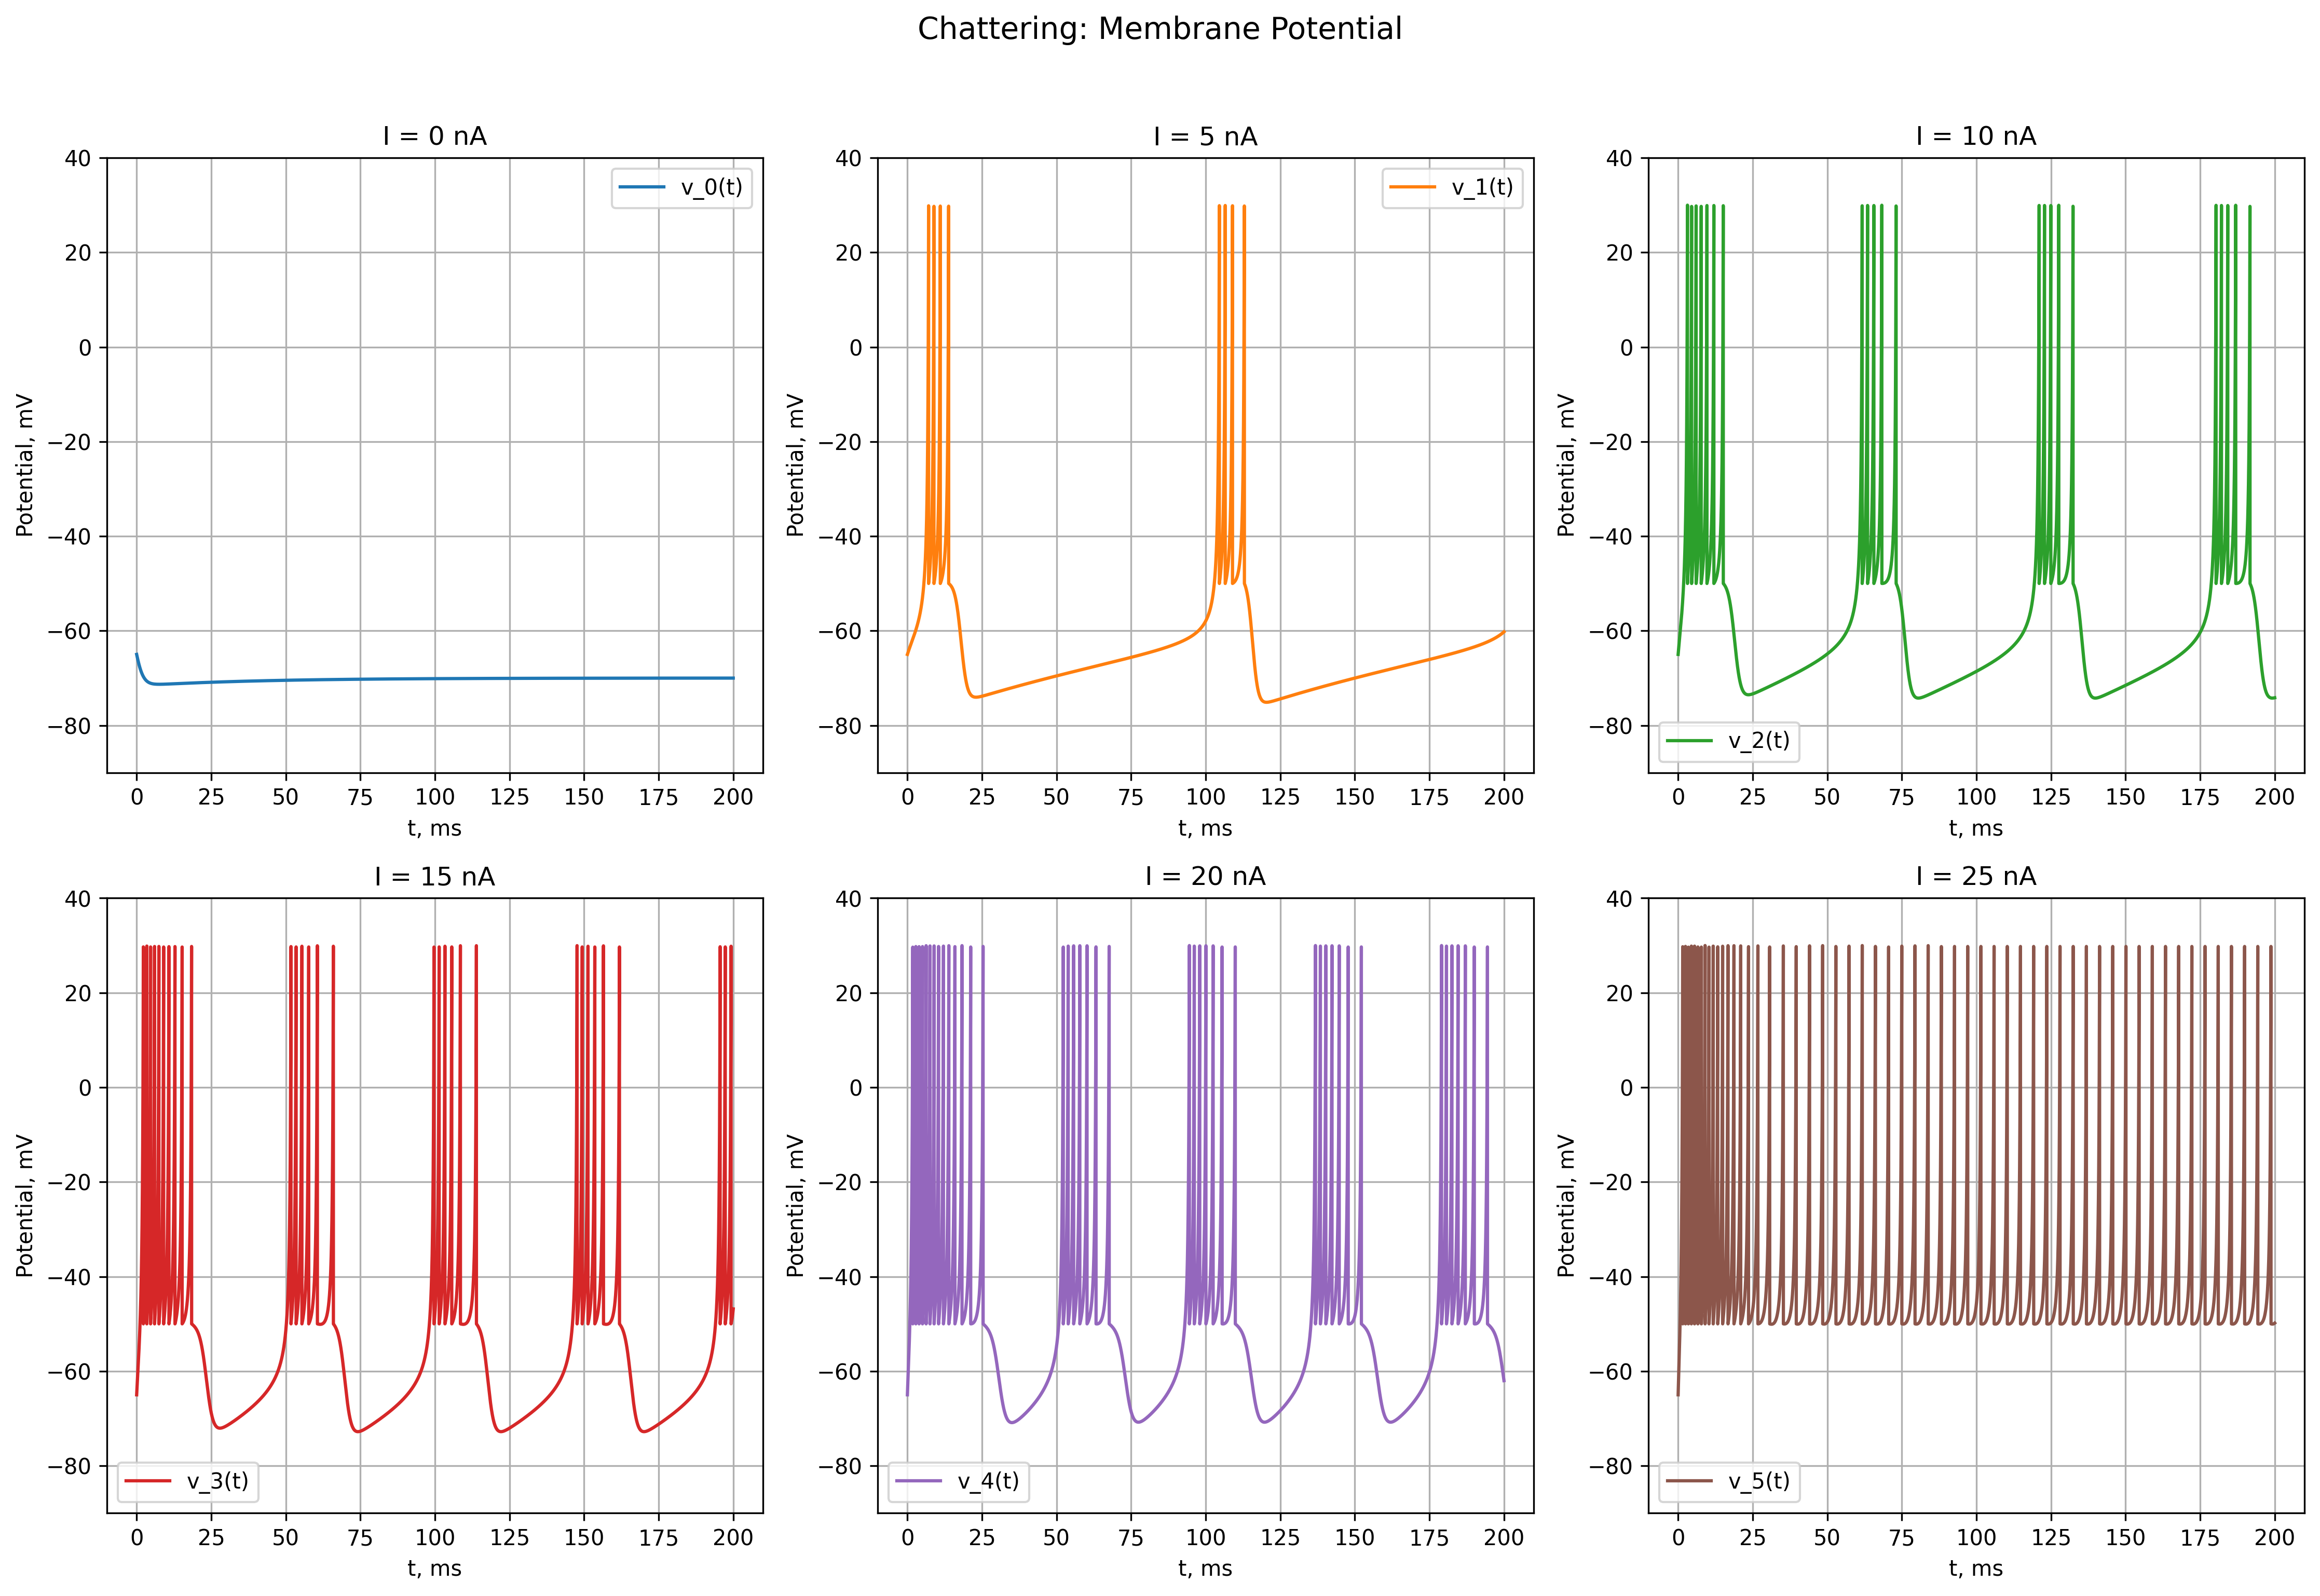
\includegraphics[width=1\linewidth]{pic/ch_different_I_potentials.png}}
	\caption{Визуализация $v(t)$ частотного нейрона для разных значений $I$.}
	\label{ch_different_I_potentials}
\end{figure}

\begin{figure}[h]
	\center{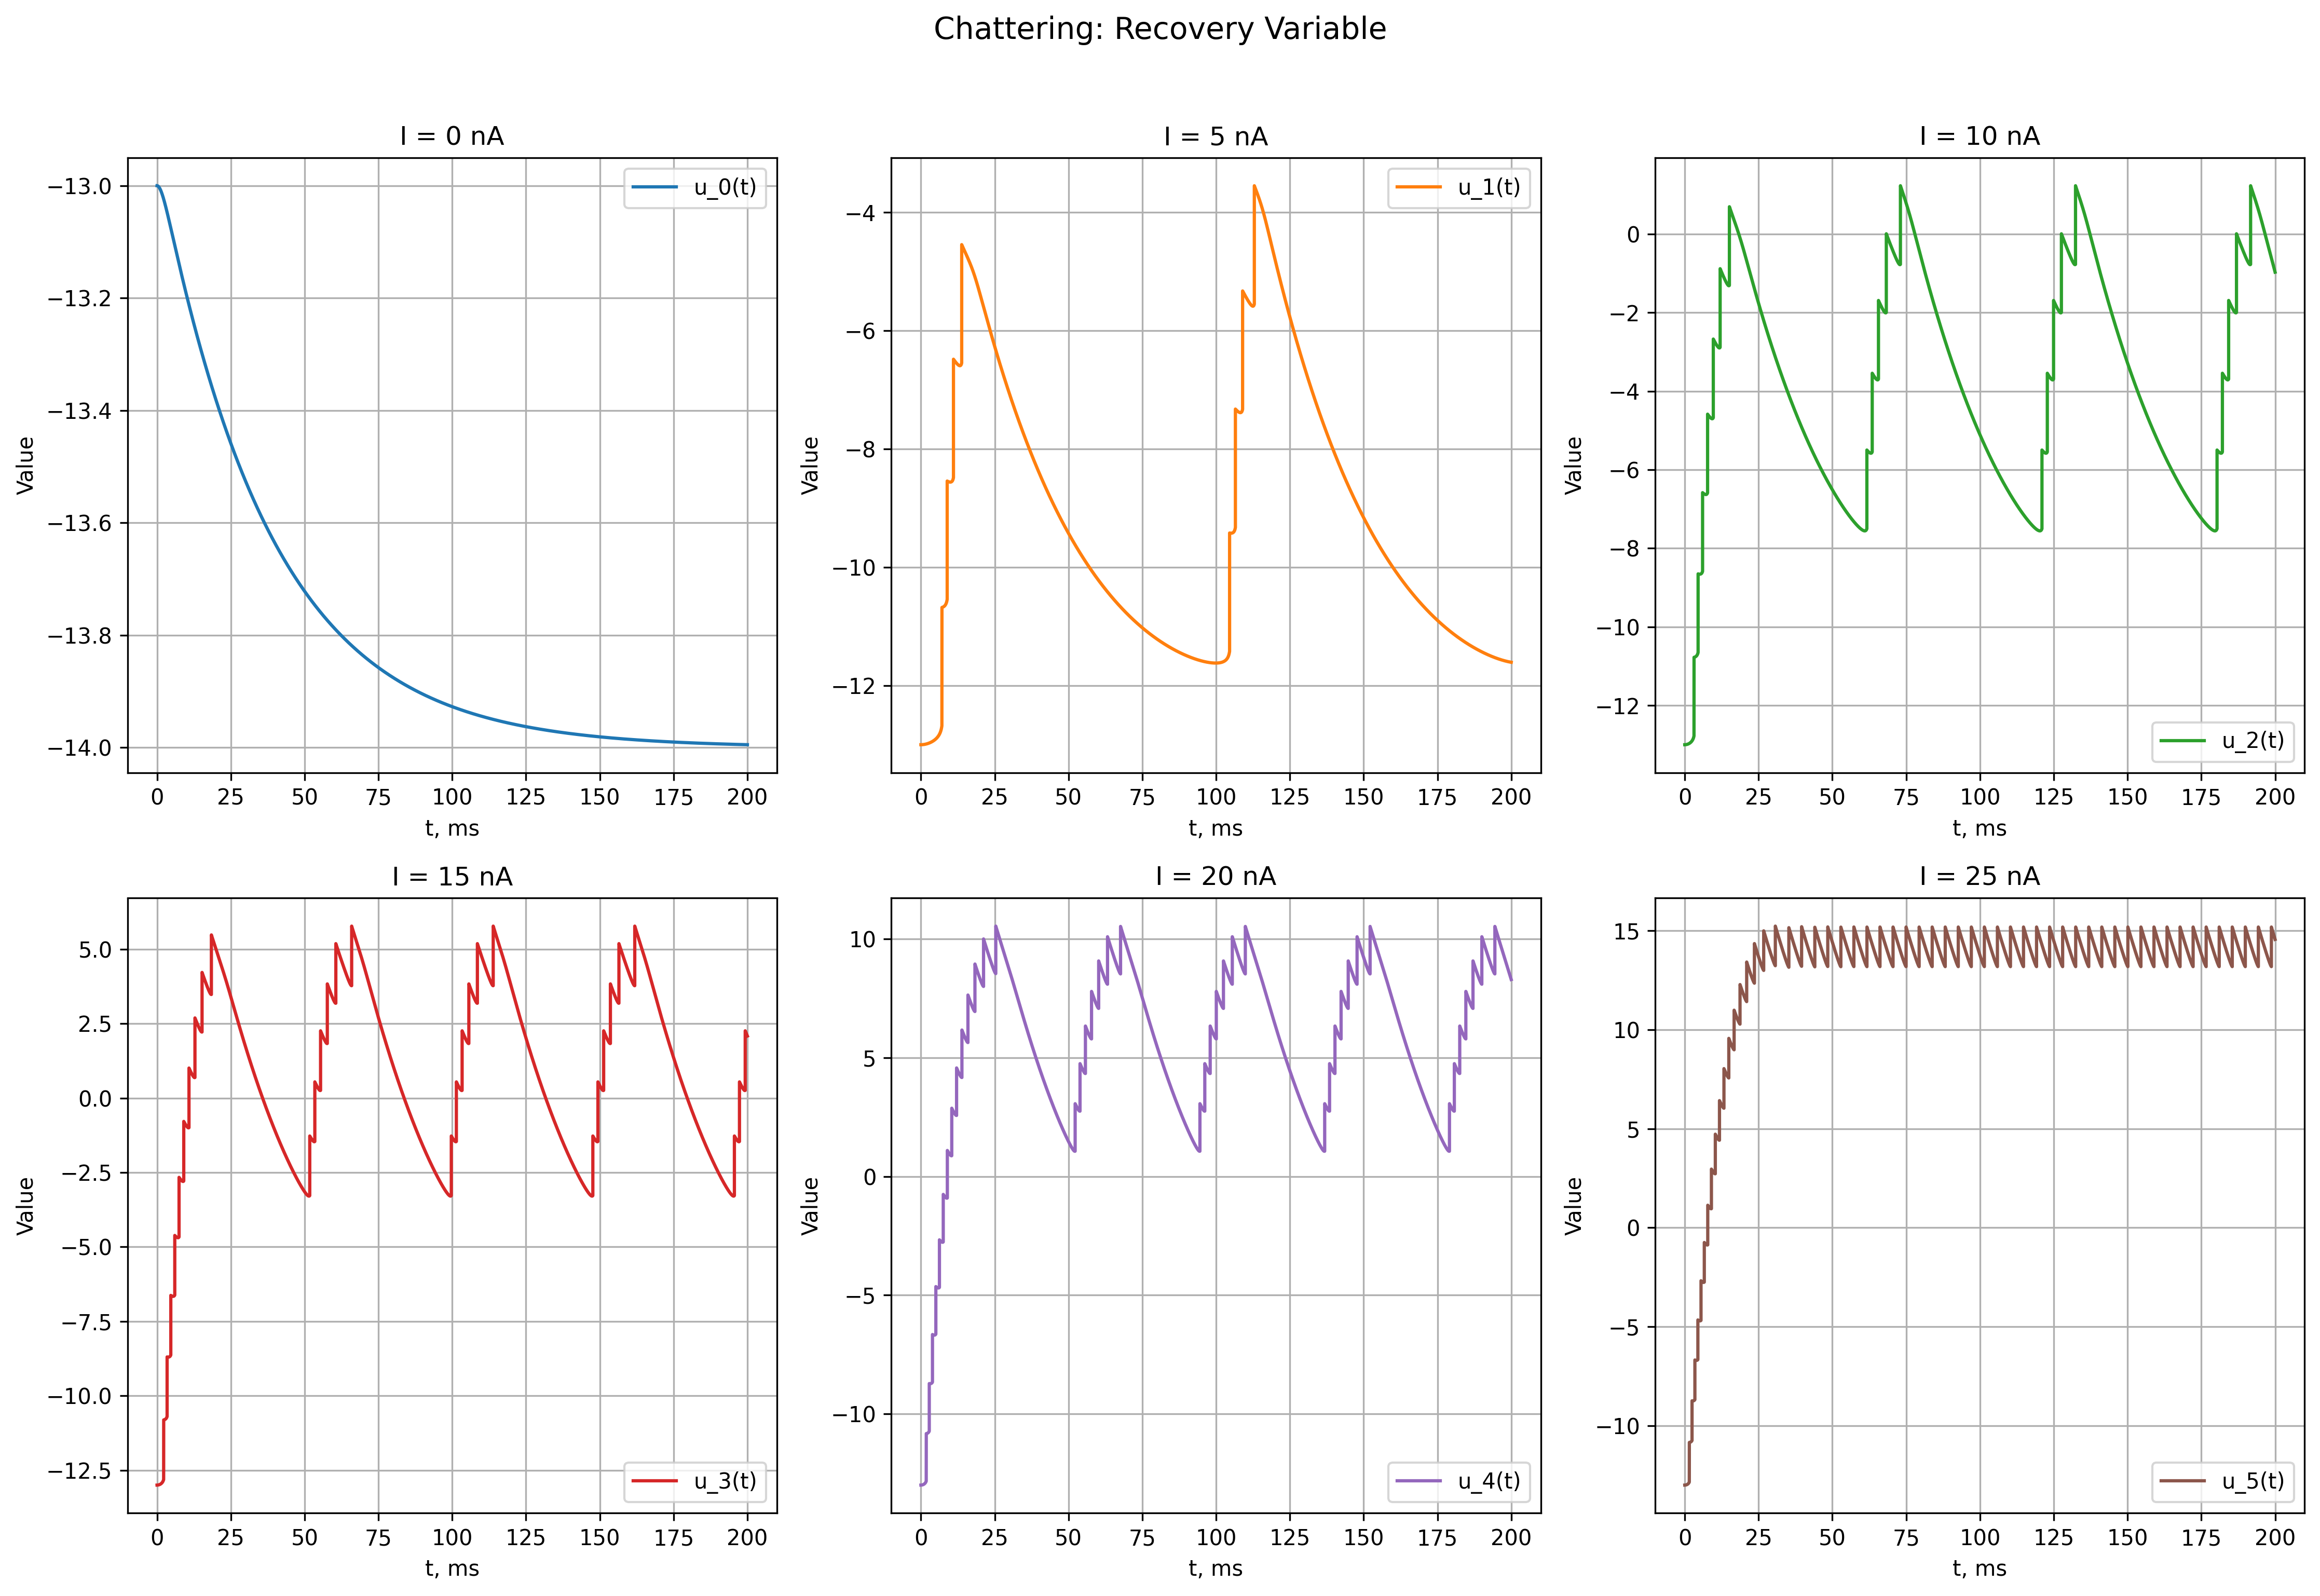
\includegraphics[width=1\linewidth]{pic/ch_different_I_recovery.png}}
	\caption{Визуализация $u(t)$ частотного нейрона для разных значений $I$.}
	\label{ch_different_I_recovery}
\end{figure}


\section{Анализ результатов}



\section{Листинг кода}

\inputminted[
breakanywhere=true, 
breaklines=true,
breaksymbolleft=\small\carriagereturn, 
frame=lines,
linenos,
fontsize=\footnotesize,
baselinestretch=0.8
]{python}{big_file.py}
\captiontextt{Листинг 1 --- Исходный код программы}





\endinput